\chapter{Introduction}
\begin{figure}[h]
\centering
\includegraphics[scale=0.35]{./intro/Coastal_names.jpg}
\end{figure}
The coastal zone is situated between the coastline and the continental shelf, and it is territory of winds, waves and currents induced effects. The coastal zone can be divided into three regions:
\begin{itemize}
\item the \textbf{shore} and \textbf{coast zone}, that are not interested by coastal processes but by wind and waves only;
\item the \textbf{surf zone} (or upper shore-face), dominated by breaking waves and wave-induced currents;
\item The middle and lower shore-face, dominated by non-breaking waves and tide-induced and wind-induced currents.
\end{itemize}
The main hydrodynamic process in the coastal zone are wind-induced and tidal waves and tidal and wind-induced currents. 
\begin{figure}[htp]
\centering
\includegraphics[scale=0.35]{./intro/Svendsen.png}
\end{figure}
\section{Wind waves}
Wind waves are gravity waves formed by the transfer of energy from the wind to the water. Wind waves mostly grows from capillary waves up to several meters, due to the combined action of wind friction, capillary tension and pressure forcing. When wind blows over a perfectly straight oceanic surface it will transfer some momentum with the friction, eventually generating a small perturbation on the surface, called capillary wave. Capillary waves are so called because the restoring force is the surface tension, they form as the wind stretches the surface and surface tension tries to restore the original equilibrium. The deflection induces an energy transfer from the wind to the ocean as the wind now drives the crest forward, but the eddy created by the deflection over the through creates a partial vacuum that drags the crest forward and pulls the trough up, starting the oscillation. Capillary waves are almost everywhere present in the ocean surface, and eventually they will transform into wind waves.
Wind-induced waves have typical periods between 5 and 15 seconds. In shallow waters they are affected by \textbf{reflection}, \textbf{refraction}, bottom friction, \textbf{shoaling} phenomena and, in the breaker zone (or surf zone) by \textbf{breaking}. In the surf zone the wave profile is highly distorted, so we can divide the breaking zone into three areas (following \cite{BoreBascoSvendsen}) as 
\begin{itemize}
\item \textbf{Outer zone}, the breaking waves are transformed into turbulent bores with rapid transition and creation of surface rollers;
\item \textbf{Inner zone}, the potential energy of the wave height is transformed in kinetic energy, then transferred and converted in roller, and finally dissipated in the small scale vortexes. In this area, long-shore currents and cross-shore return currents are created, and the mean-water set-up is generated;
\item \textbf{Swash zone}, the water motion is characterized by the up and down of plunging waves.
\end{itemize}
The breaking process starts when the fluid velocity of the wave crest tends to become equal to the wave propagation celerity. Three main types of breaking are distinguished, depending on the beach slope and steepness:
\begin{itemize}
\item \textbf{Spilling} breakers;
\item \textbf{Plunging} breakers;
\item \textbf{Surging} breakers.
\end{itemize}
\section{Tidal waves}\label{Tide}
Tides are one of the main processes that molds the coastal zone. They originate from the attraction of the earth and its hydrosphere by the sun and the moon. Their magnitude results from the relative positions of the earth,sun and moon and also the seasonal earth orientation affects the tide level. Tidal fluctuations generate currents that erode, transport and deposit materials in the coast so their action contributes to the morphology of the coastal appearance. The drivers of the Tidal wave can be summarized in:
\begin{itemize}
\item{\textit{Gravitational attraction}}: it is proportional to the mass of the two bodies and inversely related to the square of the distance between them. So, even if the Sun has a mass $27 * 10^6$ times than that of the Moon, its distance with respect to the Earth is about 400 times than that of the Earth's satellite. This explains why the Sun's tidal influence is about one half than that of the Moon.
\item{\textit{Centrifugal force}}: it originates from the interactions in the Earth-Sun-Moon system and it is the same at all Earth's locations. While the gravitational attraction differs from point to point on the Earth's surface. This generates a tide which causes the regular changes in the sea level. 
\item{\textit{Cyclic movements of the Earth and the Moon}}: the period of the Moon Orbit around the Earth is 27.3 days, the rotation of the Earth is 24 hours, so the relative period of the Earth's rotation relative to the Moon is 24 hours and 50 minutes, which is the Lunar day. This cycle movement produce the well known semidiurnal tidal cycle of 12 hours and 25 minutes. 
\item{\textit{Moon's orbit}}:
\subitem{Inclination}: of 25$^\circ$ with respect to the equator, thus tidal effects are not equally distributed around the globe
\subitem{Eccentricity}: which makes the Moon's orbit to be ellyptical so that the differences between apogee and perigee Moon distance can be about 40$\%$. 
\subitem{Earth-Moon-Sun Alignment}: produces the differentiation between \textit{spring tides} (Moon and Sun aligned with Earth) and \textit{neap tides} (Moon and Sun at 90$^\circ$ to the Earth). 
\item{\textit{Earth's irregularities}}: like basins or oddly shaped land masses, produce a system of forced waves which moves regularly from a point to another point in a given basin.
\item{\textit{Coriolis Force}} which interacts with the local basins and cause the generation of the \textit{Anphydromic systems}. Indeed as the Earth rotates and the tidal waves propagates, the Coriolis force deflects the tidal bulge from the North to the West and from the South to the West, resulting in a rotation of the tidal bulge around a central in which minimal water level takes place (i.e. the \textit(andphydromic points)).  
\end{itemize}

\subsection{Tidal bulge expression}
\begin{figure}[t]
\centering
  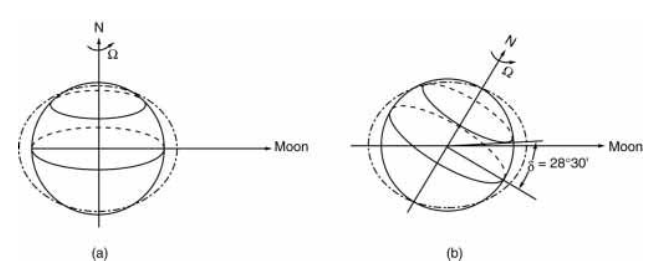
\includegraphics[scale=0.55]{./SurfWaves_figs/declination.png}
  \captionof{figure}{Declination of the moon, image from Dean-Dalrymple}
\end{figure}
By Equilibrium Theory of tides, the expression of the tidal bulge for a thin fluid layer, which lays uniformly on the Earth's surface and is subjected to the only presence of the Moon, is given by the formula:
\[
\eta_m = \frac 1 4 \frac {m_l} {m_E} r \sin^3[\pi_m (3 \cos(2 \theta_m) + 1)]
\]
where $\pi_m$ is the Moon's horizontal parallax defined by $\sin(\pi_m) = \frac r R $, $r$ is the Earth radius, $R$ is the mean Earth-Moon distance, $m_l$ and $m_E$ are respectively the masses of the Moon and the Earth, finally $\eta_m $ is the vertical water elevation due to the Moon's effect. A similar expression holds also for the Sun's effect. 

This expression is particularly important because it directly implies that the point of the Earth's surface which is mostly close to the Moon experiences the same tidal bulge than the point located on the opposite side of the Earth. 

\subsection{Why is the actual tide different?}
This is due to the fact the so called \textit{Storm-Metereologic tides} have to be accounted for. They are quite unpredictable and as important as the predictable astronomical tides.  They are characterized by a great spectrum and their contribute to the observed tides can be easily separated from the astrononomical ones.


\section{Meteorologically induced waves}\label{meteo}
The storm surges are oscillations of the water level in the coastal areas, resulting from weather perturbations, resulting typically from low atmospheric pressure conditions together with the action of the related winds, which produce storms. The wind in contact with the sea surface generates a great amount of friction, this energy transfer generates waves and pushes the water in the wind direction. If the wind direction is oriented to the coast, the related tide storm can increase the water level of several meters. They have period ranges from minutes to days. Two main types of forcing are considered.
\subsubsection*{Barometric tide}
\begin{figure}[t]
\centering
\begin{minipage}{.45\textwidth}
 \flushleft
  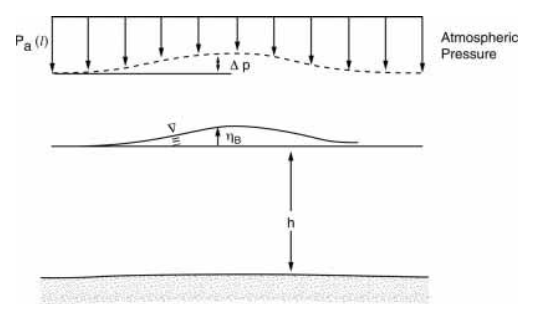
\includegraphics[scale=0.35]{./SurfWaves_figs/Barometric.png}
  \captionof{figure}{Barometric tide, image from Dean-Dalrymple}
  \label{fig:test1}
\end{minipage}%
\begin{minipage}{.45\textwidth}
  \centering
  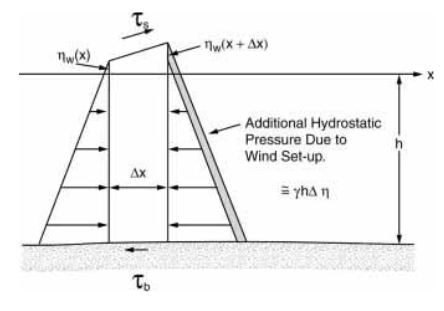
\includegraphics[scale=0.35]{./SurfWaves_figs/wind_setup.png}
  \captionof{figure}{Wind induced set-up, image from Dean-Dalrymple}
  \label{fig:test2}
\end{minipage}
\end{figure}
Due to the low pressure generating the storm, the barometric tide is the water level adjustment due to this pressure difference. A simplified approach to evaluate the magnitude of the barometric tide relies on the hydrostatic pressure equivalence. Comparing the hydrostatic pressure inside the storm and outside the storm, a first glimpse on the elevation of the mean-water level $\eta_{B}$ can be obtained by
\begin{equation}
\underbrace{p_{atm}+\gamma h}_{\text{\tiny outside}}=\underbrace{p_{atm}+\gamma \rbkt{h+\eta_{B}}-\Delta p}_{\text{\tiny outside}}
\end{equation}
thus giving a first relation for $\eta_{B}$ as
\begin{equation}
\eta_{B}=\dfrac{\Delta p}{\gamma}.
\end{equation}
Here, $\Delta p$ is the pressure difference with respect to the atmosferic pressure $p_{atm}$ and $\gamma$ is the specific weight of the water.
\subsubsection*{Wind set-up}
The frictional drag created by the wind on the surface of the sea increases the mean-water level. This increase is due to the \textit{wind stress}, that is a horizontal stress per unit area exerted on the water surface. The empirical formula is
\begin{equation}
\tau_{w}=\rho c_{f} W^{2}
\end{equation}
where $\rho$ is the density of the water (not of the air), $W$ is the wind velocity and $c_{f}$ is a dimensionless frictional coefficient, spanning from $1.2\times10^{-6}$ (low winds perturbs less the water surface) to $3.4\times10^{-6}$ (high speed winds perturbs more the surface and the roughness increases). A simple one dimensional model to evaluate the wind set-up is obtained by comparing the forces operating on a control volume of width $\Delta x$ and boundaries with height $\eta_{w}$ and $\eta_{w}+\Delta\eta$ respectively. The forces acting on this control volume, assuming hydrostatic conditions, are
\begin{equation*}
\dfrac{1}{2}\rho g \eta_{w}^{2}-\dfrac{1}{2}\rho g\rbkt{ \eta_{w}+\Delta\eta}^{2}+\tau_{s}\Delta x-\tau_{B}\Delta_{x}=0
\end{equation*}
Assuming that $\Delta\eta$ is small enough to be neglected when appearing at a second power, a first order evaluation of the wind set-up is given by
\begin{equation}
\Delta\eta=\dfrac{\tau_{s}-\tau_{B}}{\rho g \eta_{w}}\Delta x
\end{equation}
\subsubsection*{Questions}
\begin{itemize}
\item What is coastal flooding hazard. What are the drivers that cause coastal flooding.
\item What is the effect of “Climate change” or “Global Warming” on sea level rise
\item What are the possible Mitigation measures for Coastal flooding (structural and non-structural. Hint: see lesson 12)
\item What is the Tide? What are the drivers and what is the bulge shape (no demonstration, just physical meaning)? Why is the actual tide different? See Section \ref{Tide}
\item What is the tidal force (at the base of the equilibrium theory of tides). See Section \ref{Tide}
\item Describe how to predict the tide. See Section \ref{Tide}
\item How do you evaluate the barotropic component of surge. See Section \ref{meteo}
\item What is the balance that defines the wind-setup? See Section \ref{meteo}
\item What is Wind setup, Surge in general? What are the equation in Stationary conditions? See Section \ref{meteo}
\end{itemize}
\chapter{Waves theory}

\section{Wave design}
A "periodic surface gravity wave of permanent form" propagating over a horizontal bottom is fully characterized by:
\begin{itemize}
\item the wave \textbf{height} $H$;
\item the wave \textbf{length} $L$;
\item the mean-water \textbf{depth} $h$.
\end{itemize}
The crest height is the distance between the mean-water level (\textbf{mwl} or \textbf{swl}, surface water level) and the highest point of the wave (the crest), and its also referred as the positive wave amplitude. Similarly, the trough depth, or negative wave amplitude, is the distance between the mwl and the lowest point of the wave (the trough). In the context of linear wave theory, these two amplitudes are equal, and we shall refer to them simply as "amplitude", $a=H/2$. At a fixed point in space, the time between the passing of two crests, and thus of a single wave, is the \textbf{wave period} $T$. At such a point, the phase is zero under the crest and $\pi$ under the trough. Considering a two dimensional (spatial) wave, in the horizontal plane connecting the curve connecting adjacent crest points is called wave front. More generally, the wave front is defined as a curve of constant phase. The direction of the wave is described by the \textbf{waves orthogonals}, which are the orthogonal trajectories to the wave front. A progressive wave is a unidirectional wave train (i.e. there is no reflection phenomena). The front propagates with celerity (or phase velocity) $\mathbf{c}$ in the orthogonal direction. For small waves (i.e. the framework of linear theory) the wave energy $E$, composed by a potential and a kinetic part, propagates with group celerity $c_{g}$ in the same direction. The wave power, or energy flux, is $P=c_{g} E$. A progressive wave transports energy and momentum, but not necessarily mass: to understand whether we have to analyse the particle motion from top to bottom. Defining the volume flux $q$ as 
\begin{equation}
q=\dfrac{1}{T}\int_{0}^{h}u\rbkt{z}\,dz
\end{equation}
that is (one) temporal average of the velocity $u$ of the fluid particles. If $q=0$ then the motion is of pure wave. In the linear theory particles orbits are closed curves. At the mean-water level the vertical axis is equal to $H/2$, while at the bottom the trajectory degenerates to a straight line. In deep water particles move in circles, while in shallow water the ellipses are much stretched horizontally. The particle velocity $u$ is in the direction of the celerity under the crest, counter directional under the trough. The particle speed is usually much smaller than the celerity, that is $u<<c$, but the particle grows in the vicinity of the crest, where $u\equiv c$. The wave \textbf{steepness} $S$ is defined as the ratio between the wave height and length, $S=H/L$.
\subsubsection*{Short period waves}
Wind waves and swells are characterized by a short period. Wind waves are born in the open sea, where the wind velocity near the surface exceeds the critical value of $1 m/s$. This process is called wind generation, and the result is the creation of small ripples over the surface. Under the continued action of the wind, waves gradually grows in height, length and period. Swells are similar waves but coming from distant storms or from distant wave generating areas, so they are more regular as there is no wind forcing on them. The \textbf{fetch} is the area where the wind blows over the water, so we can distinguish wind-waves from swells if they are observed inside the fetch (wind-waves) or outside (swells) but the generation process is the same.
\subsubsection*{Long period waves}
Tides and storm surges are long period waves, and they are too long to be perceived as a cyclic phenomena from the occasional observer point of view. Exceptions are Tsunamis and Harbour resonance waves, of which height can be very high.
\subsubsection*{Classification of waves}
\begin{figure}[b]
\centering
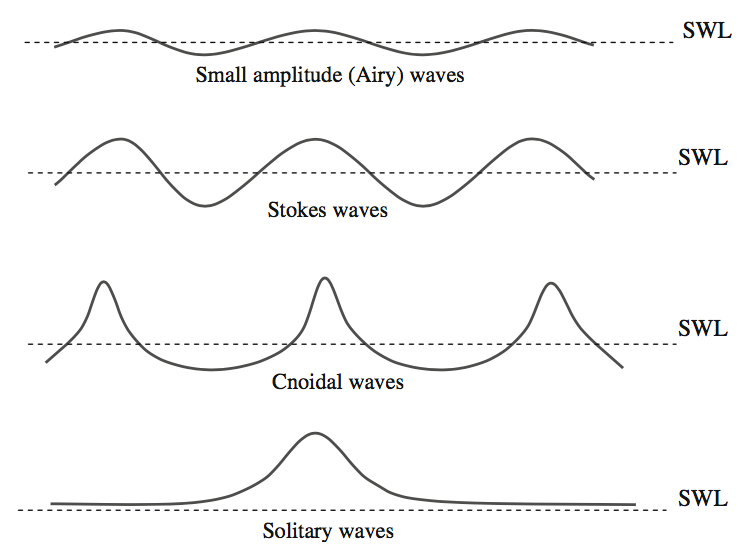
\includegraphics[scale=0.25]{./SurfWaves_figs/Type_of_waves.png}
\caption{Different types of waves, picture taken from}
\end{figure}
The general theory lies on some classification of the waves based on geometric parameters rather than the previously introduced phenomenological classification. If the wave height is (infinitely) small, than means
\begin{equation}
\dfrac{H}{L}	\rightarrow 0 \, \text{ and } \, \dfrac{H}{h}\rightarrow 0
\end{equation}
we talk about small waves, small amplitude waves, infinitesimal waves, linear waves, sinusoidal waves, Airy waves, simple harmonic waves, first order Stokes waves. The wave motion is a process that is inherently non-linear, but for small amplitude waves this non-linearity is not pronounced. However, if the non-linearity is visible, we talk about finite amplitude waves, likes Stokes waves or cnoidal waves. If the wave height is comparable to the water depth, i.e.
\begin{equation}
H=\mathcal{O}\rbkt{h}
\end{equation}
then we talk about high waves. Another classification is in terms of water depth, compared to the height of the wave, as so we have
\begin{center}
\begin{tabular}{ r r c l }
Shallow water &   & $h/L$ & $<1/20$ \\ 
Intermediate water & $1/20<$ & $h/L$ & $<1/2$ \\  
Deep water & $1/2 <$ & $h/L$. &      
\end{tabular}
\end{center}
Since the fully characterization of a wave with its length, height and water depth is possible, we can introduce the so called \textbf{Ursell parameter}
\begin{equation}
U=\dfrac{HL^{2}}{h^{3}}.
\end{equation}
Under a certain small value of the Ursell parameter, the wave will be a Stokes wave, and it could be described by Stokes theory. If furthermore we have small amplitude, we can describe a small Ursell number wave with a linear theory. Long and high waves will have high Ursell parameter, and if it is larger than a certain figure, Stokes theory will fail and Cnoidal waves have to be introduced.
\section{Governing equations}
Referring to the usual continuum theory, that can be regarded as the hypothesis of a small volume of fluid behaving in the same manner no matter how small the volume itself is, the fluid is regarded as having the same density $\rho$, viscosity $\mu$ and temperature. The water is thus \textbf{homogeneous}. With this assumption, the usual mass conservation statement
\begin{equation}
\dfrac{d}{dt}\int_{V\rbkt{t}}\rho\rbkt{t,\mathbf{x}}\,dV\overset{Transport\text{  }Thm.}{=}\int_{V\rbkt{t}}
\dfrac{d}{dt}\rho\rbkt{t,\mathbf{x}}+\mathbf{u}\cdot\nabla\rho\rbkt{t,\mathbf{x}}\,dV =0,
\end{equation}
which has Eulerian form
\begin{equation}
\dfrac{\partial}{\partial t}\rho\rbkt{t,\mathbf{x}}+\nabla\rbkt{\mathbf{u}\rbkt{t,\mathbf{x}}\cdot\rho\rbkt{t,\mathbf{x}}}=0,
\end{equation}
can be simplified to 
\begin{equation}
\nabla\cdot\mathbf{u}\rbkt{t,\mathbf{x}}=0,
\end{equation}
as the temporal derivative of $\rho\rbkt{t,\mathbf{x}}$ is zero, as much as the spatial gradient of the density appearing by applying the chain rule to the divergence. Considering the $\rbkt{x,z}$ plane, where the wave motion has its relevant characteristics, we can express the continuity as 
\begin{equation}
\dfrac{\partial}{\partial x}u\rbkt{t,\mathbf{x}}+\dfrac{\partial}{\partial z}w\rbkt{t,\mathbf{x}}=0.
\end{equation}
The second conservation statement is the momentum balance, that is the classical Navier-Stokes equation
\begin{equation}
\rho\rbkt{\dfrac{\partial}{\partial t}\mathbf{u} + \mathbf{u}\cdot\nabla\mathbf{u}}=-\nabla p +\rho\mathbf{g}\nabla h+\mu\Delta\mathbf{u}.
\end{equation}
Neglecting the viscous term (as it is a process that enter rarely in coastal processes) we obtain Euler equation
\begin{equation}
\rho\rbkt{\dfrac{\partial}{\partial t}\mathbf{u} + \mathbf{u}\cdot\nabla\mathbf{u}}=-\nabla p +\rho\mathbf{g}\nabla h.
\end{equation}
with $\mathbf{g}=\rbkt{0,0,-g}$. In our $\rbkt{x,z}$ framework we have thus
\begin{equation}
\begin{array}{l}
\vphantom{\int^{\dfrac{1}{2}}}\dfrac{\partial u}{\partial t} + u \dfrac{\partial u}{\partial x} + w \dfrac{\partial u}{\partial z}=-\dfrac{1}{\rho}\dfrac{\partial p}{\partial x} \\
\vphantom{\int^{\dfrac{1}{2}}}\dfrac{\partial w}{\partial t} + u \dfrac{\partial w}{\partial x} + w \dfrac{\partial w}{\partial z}=-\dfrac{1}{\rho}\dfrac{\partial p}{\partial z}-g\dfrac{\partial h}{\partial z}
\end{array}
\end{equation}
Supposing constant depth, we will have $h=h\rbkt{z}=z$, so that the last derivative in the second equation will be simply equal to 1. At this point, two assumptions are embedded in our equations, the inviscid character of the flow, explicitly made with $\mu=0$, and conservativity of the external forces, lying under the Navier-Stokes equations. With these two conditions we have validity of the Kelvin circulation theorem. Evaluating the temporal variation of the circulation as
\begin{align*}
\dfrac{d\Gamma}{dt}&=\oint \dfrac{d}{dt}\rbkt{\bs{d\ell}\cdot\mathbf{u}}=\oint \dfrac{d\mathbf{u}}{dt}\cdot\bs{d\ell}+\oint\mathbf{u}\dfrac{d}{dt}\cdot\rbkt{\bs{d\ell}}\\
&=\oint d\rbkt{\bs{d\ell}}\cdot\nabla\rbkt{\dfrac{p}{\rho}+gh}+\oint \bs{d\ell}\cdot \rbkt{\nu\Delta\mathbf{u}} + \oint\mathbf{u}\cdot\rbkt{\bs{d\ell}\cdot\nabla\mathbf{u}}\\
&=\oint d\rbkt{\bs{d\ell}}\cdot\nabla\rbkt{\dfrac{p}{\rho}+gh+\dfrac{\mathbf{u}^{2}}{2}}+\nu\oint \bs{d\ell}\cdot \rbkt{\Delta\mathbf{u}}\\
&=\int_{A}\nabla\times\nabla E\cdot\mathbf{n}\, dA-\nu\oint\rbkt{\nabla\times\bs{\omega}}\bs{d\ell}\\
&=-\nu\oint\rbkt{\nabla\times\bs{\omega}}\bs{d\ell}.
\end{align*}
The last step has been obtained by neglecting $\nabla\time\nabla E$ as it is always zero for any scalar quantity. Finally, if there is no initially vorticity in an inviscid fluid ($\nu=0$), then the motions is always irrotational, as we have
\begin{equation}
\dfrac{d\Gamma}{dt}=0 \qquad \text{(Kelvin Circulation Theorem)}.
\end{equation}
This irrotationality condition is important as a velocity potential function $\varphi$ can be introduced, to reduce the dimension of the problem from $\rbkt{u,w,p}$ to $\rbkt{\varphi,p}$. The potential function is defined as
\begin{equation}
\mathbf{u}=\text{grad}\rbkt{\varphi}, \quad \text{ or } \rbkt{u,w}=\rbkt{\dfrac{\partial\varphi}{\partial x},\dfrac{\partial\varphi}{\partial z}}
\end{equation}
where $\varphi$ is the potential function. Existence of this function is implied by irrotationality, as in two dimensions it holds
\begin{equation*}
\bs{\omega}=\nabla\times\mathbf{u}=\dfrac{\partial u}{\partial z}-\dfrac{\partial w}{\partial x}=\dfrac{\partial^{2}\varphi}{\partial z\partial x}-\dfrac{\partial^{2}\varphi}{\partial x\partial z}\equiv 0,
\end{equation*}
and this is the reason why a fluid with vorticity cannot be represented by a potential function. Applying the definition of the potential function to the continuity equation the Laplace equation is obtained
\begin{equation}
\left\lbrace\begin{array}{l}
\vphantom{\int^{\dfrac{1}{2}}}\dfrac{\partial u}{\partial x}+\dfrac{\partial w}{\partial z}=0 \\
\mathbf{u}=\text{grad}\rbkt{\varphi}
\vphantom{\int^{\dfrac{1}{2}}}\end{array}\right. \qquad\rightarrow\qquad \dfrac{\partial^{2} \varphi}{\partial x^{2}}+\dfrac{\partial^{2}\varphi}{\partial z^{2}}=0.
\end{equation}
Moreover, the Euler equation can be transformed using irrotationality $\partial_{x}w=\partial_{z}u$ as 
\begin{equation*}
\begin{array}{l}
\vphantom{\int^{\dfrac{1}{2}}}\dfrac{\partial u}{\partial t} + u \dfrac{\partial u}{\partial x} + w \dfrac{\partial u}{\partial z}=-\dfrac{1}{\rho}\dfrac{\partial p}{\partial x} \\
\vphantom{\int^{\dfrac{1}{2}}}\dfrac{\partial w}{\partial t} + u \dfrac{\partial w}{\partial x} + w \dfrac{\partial w}{\partial z}=-\dfrac{1}{\rho}\dfrac{\partial p}{\partial z}-g\dfrac{\partial h}{\partial z}
\end{array} \qquad\rightarrow\qquad 
\begin{array}{l}
\vphantom{\int^{\dfrac{1}{2}}}\dfrac{\partial u}{\partial t} + \dfrac{1}{2}\dfrac{\partial}{\partial x}\rbkt{u^{2}+w^{2}}=-\dfrac{1}{\rho}\dfrac{\partial p}{\partial x} \\
\vphantom{\int^{\dfrac{1}{2}}}\dfrac{\partial w}{\partial t} + \dfrac{1}{2}\dfrac{\partial}{\partial x}\rbkt{u^{2}+w^{2}}=-\dfrac{1}{\rho}\dfrac{\partial p}{\partial z}-g\dfrac{\partial h}{\partial z}.
\end{array}
\end{equation*}
Introducing the potential function and adding $g\partial_{x}h\equiv 0$ to the first term the Euler equation can be summarized into
\begin{equation}
\nabla\rbkt{\varphi'+\dfrac{\mathbf{u}^{2}}{2}+\dfrac{p}{\rho}+gh}=0.
\end{equation}
Integrating the two components we find
\begin{equation*}
\begin{array}{l}
\vphantom{\int^{\dfrac{1}{2}}}\dfrac{\partial \varphi}{\partial t} + \dfrac{1}{2}\rbkt{u^{2}+w^{2}}+\dfrac{1}{\rho}\dfrac{\partial p}{\partial x}+gh=C\rbkt{t,z} \\
\vphantom{\int^{\dfrac{1}{2}}}\dfrac{\partial \varphi}{\partial t} + \dfrac{1}{2}\rbkt{u^{2}+w^{2}}+\dfrac{1}{\rho}\dfrac{\partial p}{\partial z}+gh=C\rbkt{t,x}
\end{array}
\end{equation*}
leading to the well known Bernoulli equation
\begin{equation}
\dfrac{\partial \varphi}{\partial t} + \dfrac{1}{2}\rbkt{u^{2}+w^{2}}+\dfrac{1}{\rho}p+gh=C\rbkt{t}.
\end{equation}
Noticing that $\varphi$ and $\varphi+\int C\rbkt{t}\,dt$ leads to the same velocity field, it can redefined as
\begin{equation}
\dfrac{\partial \varphi}{\partial t} + \dfrac{1}{2}\sbkt{\rbkt{\dfrac{\partial\varphi}{\partial x}}^{2}+\rbkt{\dfrac{\partial\varphi}{\partial z}}^{2}}+\dfrac{1}{\rho}p+gh=0.
\end{equation}
This equation emphasizes the fact that pressure acts like a reaction force of which magnitude is scaled so that the momentum balance (Newton second law) is satisfied at every point of the fluid field. It is however known that no fluid is homogeneously irrational because rotationality comes from the presence of boundaries. This boundary and its physical no-slip condition, that is the fact that a particle near the boundary must have a zero mean velocity (if the boundary is fixed, otherwise it must have the same velocity of the boundary), creates strong velocity gradients and so a rotation of the fluid is induced, among with a shear stress. This is the usual setting for the boundary layer theory, but in the case of waves there is an inversion of the velocity due to waves oscillation. This velocity inversion causes also an inversion of the boundary layer. This inversion is caused by the inversion of the pressure caused by the wave motion, with the result that particles near the bed will alternately move forward and backwards. The pressure gradient will cause a detachment of the boundary layer itself, and so it will prevent the complete development, resulting in a thinner boundary layer. Summarizing, the flow is irrotational in most of the flow field, except for a very thin layer at the bottom, where there is a small dissipation as the complete development of the boundary layer is prevented by the constant inversion of the pressure gradient on the bottom. The most dissipating process will thus be the wave breaking process. To solve the wave problem we will need boundary conditions. The bottom condition is the simple imposition of an impermeable bottom, that is 
\begin{equation}
w=0, \quad \text{ or } \dfrac{\partial\varphi}{\partial z}=0 \qquad \text{at } z=-h.
\end{equation}
The free surface condition is composed of two different conditions, a kinematic one and a dynamic one. The kinematic condition is referring to the fact that a particle on the surface must remain on the surface, parametrized by $\eta=\eta\rbkt{t,x}$. Defining the material surface as
\begin{equation}
\mathcal{F}\rbkt{t,x}=\eta\rbkt{t,x}-z
\end{equation}
the free surface condition is imposed by
\begin{equation*}
\dfrac{d\mathcal{F}}{dt}=\dfrac{\partial}{\partial t}\eta+u\dfrac{\partial}{\partial x}\eta - w =0   \qquad \text{at } z=\eta.
\end{equation*}
This condition can be better understood as follows: the linearised increment of $z$ is 
\begin{equation*}
dz=\dfrac{\partial\eta}{\partial t}dt+\dfrac{\partial\eta}{\partial x}dx
\end{equation*}
but the infinitesimal displacements can be also expressed as
\begin{equation*}
\left\lbrace\begin{array}{l}
dx=udt\\
dz=wdt
\end{array}\right.
\end{equation*}
so that 
\begin{equation}
wdt=\dfrac{\partial\eta}{\partial t}dt+\dfrac{\partial\eta}{\partial x}udt    \quad \rightarrow   \quad 
w=\dfrac{\partial\eta}{\partial t}+\dfrac{\partial\eta}{\partial x}u   \qquad  \text{ at } z=\eta.
\end{equation}
In the potential form it can be also written as
\begin{equation}
\dfrac{\partial\varphi}{\partial z}=\dfrac{\partial\eta}{\partial t}+\dfrac{\partial\varphi}{\partial x}\dfrac{\partial\eta}{\partial x}   \qquad  \text{ at } z=\eta.
\end{equation}
The second condition, the dynamic one, imposes that the pressure on the surface must be that of the environment, that means $p=p_{atm}$ at $z=\eta$. As usually the pressure taken into account is a relative pressure and the effects of pressure variations between crest and trough can be neglected, the condition can be settled as $p=0$ at $z=\eta$, explicitly
\begin{equation}
g\eta + \dfrac{1}{2}\sbkt{\rbkt{\dfrac{\partial\varphi}{\partial x}}^{2}+\rbkt{\dfrac{\partial\varphi}{\partial z}}^{2}} +\dfrac{\partial \varphi}{\partial t}=0\qquad  \text{ at } z=\eta.
\end{equation}
\section{Linear theory (Airy waves)}\label{Airy}
Fundamental hypothesis of the linear theory are:
\begin{itemize}
\item It's considered the case of constant water depth $h$ and constant wave period $T$; 
\item Two dimensional motion is assumed: essentially the wave height is assumed constant among the wave front.
\end{itemize}
Attention must be posed on the fact that these two assumptions excludes wind waves inside the fetch.
\begin{itemize}
\item Constant shape of the wave, meaning that there are no changes in the form of the wave. Mathematically speaking, the motion is steady;
\item Incompressibility of the fluid is assumed, that is constant density. Although the limit of velocity for water to be considered incompressible is $1500m/s$, much faster than the usual waves speed, when the wave breaks it becomes a mixture of water and air, thus this high presence of compressible gases make this hypothesis no more valid. Far from breaking situations, incompressibility holds;
\item In between some specific boundaries for $L/h$ and $H/h$ the effects of viscosity and turbulence in the boundary layer can be neglected. Outside these boundaries they cannot be neglected, as indeed the thickness is proportional to $H$ and $L$. For tidal waves and tsunamis the boundary layer plays a non negligible role.
\end{itemize}
The governing equations are
\renewcommand{\arraystretch}{2.5}
\begin{equation*}
\begin{array}{ll}
\dfrac{\partial^{2} \varphi}{\partial x^{2}}+\dfrac{\partial^{2}\varphi}{\partial z^{2}}=0 & \\
p=-gh - \dfrac{1}{2}\sbkt{\rbkt{\dfrac{\partial\varphi}{\partial x}}^{2}+\rbkt{\dfrac{\partial\varphi}{\partial z}}^{2}} -\dfrac{\partial \varphi}{\partial t} & \\
\dfrac{\partial\varphi}{\partial z}=0 & \text{at } z=-h\\
\dfrac{\partial\varphi}{\partial z}=\dfrac{\partial\eta}{\partial t}+\dfrac{\partial\varphi}{\partial x}\dfrac{\partial\eta}{\partial x}   \qquad  & \text{ at } z=\eta \\
g\eta + \dfrac{1}{2}\sbkt{\rbkt{\dfrac{\partial\varphi}{\partial x}}^{2}+\rbkt{\dfrac{\partial\varphi}{\partial z}}^{2}} +\dfrac{\partial \varphi}{\partial t}=0 & \text{ at } z=\eta
\end{array}
\end{equation*}
where $\eta$ and $z$ are measured at the mean water level, defined as 
\begin{equation}
\int_{0}^{L}\eta\rbkt{t,x}\,dx=0.
\end{equation}
This system of equations still presents two mathematical difficulties, the non linearity in the boundary conditions and the fact that $\eta$ is actually unknown. Without any further simplification this problem is (analytically) unsolvable. To simplify the problem a dimensional analysis is performed. Deep water waves are considered, of which particles are moving in a circle-like motion. Due to the free surface condition, imposing that the particles on the surface will remain on the surface, these particles will move with a period $T$ over an orbit of vertical axis length $H$. The speed of the particle can be approximated by $V=\pi H/T$, meaning that 
\begin{equation*}
u_{max}=w_{max}=\dfrac{\partial\varphi}{\partial x}=\dfrac{\partial\varphi}{\partial z}=\dfrac{\pi H}{T}=\mathcal{O}\rbkt{\dfrac{H}{T}}
\end{equation*}
and similarly
\begin{align*}
\dfrac{\partial\eta}{\partial t}&=\dfrac{H}{T/2}=\mathcal{O}\rbkt{\dfrac{H}{T}} \\
\dfrac{\partial\eta}{\partial x}&=\dfrac{H}{L}=\mathcal{O}\rbkt{\dfrac{H}{L}}
\end{align*}
and the celerity can be estimated by $c=H/T$. The kinematic boundary condition can be analysed by meaning of its components order of magnitude
\begin{align*}
\dfrac{\partial\eta}{\partial t}&=\mathcal{O}\rbkt{\dfrac{H}{T}}=\mathcal{O}\rbkt{\varphi_{z}} \\
\dfrac{\partial\varphi}{\partial x}\dfrac{\partial\eta}{\partial t}&=\mathcal{O}\rbkt{\dfrac{H}{T}}\mathcal{O}\rbkt{\dfrac{H}{L}}=\mathcal{O}\rbkt{c\dfrac{H^{2}}{L}}=\dfrac{H}{L}\mathcal{O}\rbkt{\varphi_{z}} \\
\end{align*}
thus if $H/L\rightarrow 0$ the kinematic boundary condition can be linearised, as far as the non-linear dynamic condition for the pressure. The results are
\renewcommand{\arraystretch}{2.5}
\begin{equation*}
\begin{array}{ll}
\dfrac{\partial\varphi}{\partial z}-\dfrac{\partial\eta}{\partial t}=0  & \text{ at } z=\eta. \\
\eta + \dfrac{1}{g}\dfrac{\partial \varphi}{\partial t}=0 & \text{ at } z=\eta.
\end{array}
\end{equation*}
With this approach also the unknownness of $\eta=\eta\rbkt{t,x}$ can be tackled. Expanding in Taylor series the velocity $w$ 
\begin{align*}
w\rbkt{t,x,\eta}&=\dfrac{\partial\varphi}{\partial z}\rbkt{t,x,\eta}=\dfrac{\partial\varphi}{\partial z}\rbkt{t,x,0}+\eta\dfrac{\partial^{2}\varphi}{\partial z^{2}}\rbkt{t,x,0}+...\\
&=\dfrac{\partial\varphi}{\partial z}\rbkt{t,x,0}-\eta\dfrac{\partial^{2}\varphi}{\partial x^{2}}\rbkt{t,x,0}+...
\end{align*}
by mean of the Laplace equation, while exploiting 
\begin{equation*}
\eta=\mathcal{O}\rbkt{H} \qquad \text{and} \qquad \dfrac{\partial^{2}\varphi}{\partial x^{2}}\mathcal{O}\rbkt{\dfrac{1}{L}\dfrac{\partial\varphi}{\partial x}}
\end{equation*}
the second order term can be compared to
\begin{equation*}
\eta\dfrac{\partial^{2}\varphi}{\partial x^{2}}=\mathcal{O}\rbkt{\dfrac{H}{L}\varphi_{z}}
\end{equation*}
and thus for $H/L\rightarrow 0$ the velocity can be approximated as
\begin{equation}
w\rbkt{t,x,\eta}=w\rbkt{t,x,0}.
\end{equation}
Similar result holds for $\partial\varphi/\partial t$, and both can be evaluated at $z=0$ instead of at $z=\eta$ with first order accuracy. The mathematical problem under \textbf{small waves hypothesis} $H/L\rightarrow 0$ is finally
\renewcommand{\arraystretch}{2.5}
\begin{equation*}
\begin{array}{ll}
\dfrac{\partial^{2} \varphi}{\partial x^{2}}+\dfrac{\partial^{2}\varphi}{\partial z^{2}}=0 & \\
\dfrac{\partial\varphi}{\partial z}=0 & \text{at } z=-h.\\
\dfrac{\partial\varphi}{\partial z}-\dfrac{\partial\eta}{\partial t}=0  & \text{ at } z=0 \\
\eta + \dfrac{1}{g}\dfrac{\partial \varphi}{\partial t}=0 & \text{ at } z=0
\end{array}
\end{equation*}
\renewcommand{\arraystretch}{1}
among with the periodicity condition
\begin{equation*}
\dfrac{\partial\varphi}{\partial x}\rbkt{t,0,z}=\dfrac{\partial\varphi}{\partial x}\rbkt{t,L,z}
\end{equation*}
representing the boundary condition in the $x-$dimension. Since $\eta$ does not appear in the Laplace equation it can be eliminated from the problem deriving in $t$ the free surface dynamic condition and substituting it in the kinematic condition 
\begin{equation*}
\begin{array}{ll}
\dfrac{\partial \varphi}{\partial z} + \dfrac{1}{g}\dfrac{\partial^{2} \varphi}{\partial t^{2}}=0 & \text{ at } z=0.
\end{array}
\end{equation*}
\subsection{Solution for waves of constant form}\label{solution}
The simplification of constant form waves is of paramount importance; supposing that the wave has length $L$ and constant period $T$ the celerity is $c=L/T$. The constant form assumption requires that
\begin{equation*}
\eta\rbkt{x_{0},t_{0}}=\eta\rbkt{x_{1},t_{1}}
\end{equation*}
for two points related by 
\begin{equation*}
x_{1}=x_{0}+c\rbkt{t_{1}-t_{0}} \qquad \text{ with} t_{1}-t_{0}=T
\end{equation*}
that is
\begin{equation*}
\dfrac{x_{1}-x_{0}}{L}=\dfrac{t_{1}-t_{0}}{T}.
\end{equation*}
A normalized variable
\begin{equation}
\theta=2\pi\rbkt{t/T-x/L}
\end{equation}
can be introduced, so that
\begin{align*}
\eta\rbkt{t,x}&\rightarrow \eta\rbkt{\theta}\\
\varphi\rbkt{t,x,z}&\rightarrow \varphi\rbkt{\theta,z}
\end{align*}
resulting in 
\begin{align*}
\dfrac{\partial^{2}}{\partial x^{2}}\varphi\rbkt{t,x,z}&=\dfrac{\partial^{2}}{\partial x^{2}}\varphi\rbkt{\theta,z}=\dfrac{\partial}{\partial x}\sbkt{\dfrac{\partial}{\partial x}\varphi\rbkt{\theta,z}}=\dfrac{\partial}{\partial x}\sbkt{\dfrac{\partial\varphi}{\partial\theta}\dfrac{\partial\theta}{\partial x}}=\dfrac{2\pi}{L}\sbkt{\dfrac{\partial}{\partial\theta}\dfrac{\partial\varepsilon}{\partial x}}\\
&=\rbkt{\dfrac{2\pi}{L}}^{2}\dfrac{\partial^{2}\varphi}{\partial\theta^{2}}
\end{align*}
and hence introducing the parameter $k=2\pi/L$ the Laplace equation becomes anisotropic and can be written as
\begin{equation}
k^{2}\dfrac{\partial^{2}\varphi}{\partial\theta^{2}}+\dfrac{\partial^{2}\varphi}{\partial z^{2}}=0.
\end{equation}
Similarly, introducing the parameter $\omega=2\pi/T$ the free surface condition can be written as
\begin{equation}
\begin{array}{ll}
\dfrac{\partial\varphi}{\partial z}+\dfrac{\omega^{2}}{g}\dfrac{\partial^{2}\varphi}{\partial\theta^{2}}=0 & \text{ at } z=0,
\end{array}
\end{equation}
while the periodicity condition is simply
\begin{equation*}
\varphi_{\theta}\rbkt{0,z}=\varphi_{\theta}\rbkt{-2\pi,z}.
\end{equation*}
Of course the variable $\theta$ can be written any time with respect to $\omega$ (frequency) and $k$ (wave number) as
\begin{equation}
\theta=\omega t -kx.
\end{equation}
This formulation can be solved with the separation of variables technique, that is expressing the potential $\varphi$ as
\begin{equation}
\varphi\rbkt{\theta,z}=f\rbkt{\theta}Z\rbkt{z}
\end{equation}
so that the Laplace equation becomes 
\begin{equation*}
k^{2}f''\rbkt{\theta}Z\rbkt{z}+f\rbkt{\theta}Z''\rbkt{z}=0
\end{equation*}
that is
\begin{equation*}
-k^{2}\dfrac{f''\rbkt{\theta}}{f\rbkt{\theta}}=\dfrac{Z''\rbkt{z}}{Z\rbkt{z}}
\end{equation*}
but being the right hand side and the left hand side functions of two different independent variables, they can be identically equal only if and only if they are identically equal to a constant, that is
\begin{equation*}
-k^{2}\dfrac{f''\rbkt{\theta}}{f\rbkt{\theta}}=\lambda^{2}\qquad\dfrac{Z''\rbkt{z}}{Z\rbkt{z}}=\lambda^{2}
\end{equation*}
with $\lambda\in\R$. The problem has thus been transformed into a system of ODEs
\begin{equation}
\left\lbrace\begin{array}{l}
f''\rbkt{\theta}+\dfrac{\lambda^{2}}{k^{2}}f\rbkt{\theta}=0 \\
Z''\rbkt{z}-\lambda^{2}Z\rbkt{z}=0.
\end{array}\right.
\end{equation}
Since the first equation is an harmonic oscillator while the second is an harmonic repulsor the solution can be expressed as
\begin{equation}
\left\lbrace\begin{array}{l}
f\rbkt{\theta}=A\cos\rbkt{\dfrac{\lambda}{k}\theta}+B\sin\rbkt{\dfrac{\lambda}{k}\theta}=C\sin\rbkt{\dfrac{\lambda}{k}\theta+\delta}\\
Z\rbkt{z}=D\cosh\rbkt{\lambda z}+E\sinh\rbkt{\lambda z}.
\end{array}\right.
\end{equation}
The search of the constants starts with the periodicity condition
\begin{equation*}
\varphi_{\theta}\rbkt{0,z}=\varphi_{\theta}\rbkt{-2\pi,z}.
\end{equation*}
that becomes
\begin{equation*}
f'\rbkt{0}=f'\rbkt{-2\pi} \quad\rightarrow\quad \sin\rbkt{\delta}=\sin\rbkt{-\dfrac{\lambda}{k}2\pi+\delta}
\end{equation*}
that implies that $\lambda/k=1$. Using $\varphi\rbkt{\theta,z}=f\rbkt{\theta}Z\rbkt{z}$ at the bottom, with the condition $w=0$ for $z=-h$, from the second equation it can be gained the relation 
\begin{equation*}
D\cosh\rbkt{-k h}+E\sinh\rbkt{-k h}=0
\end{equation*}
that is 
\begin{equation*}
D=E\coth\rbkt{k h}
\end{equation*}
and thus $Z\rbkt{z}$ can be defined as
\begin{align*}
Z\rbkt{z}&=E\coth\rbkt{k h}\cosh\rbkt{k  z}+E\sinh\rbkt{k  z}\\
&=\dfrac{E}{\sinh\rbkt{k h}}\sbkt{\cosh\rbkt{k  h}\cosh\rbkt{k  z}+\sinh\rbkt{k  h}\sinh\rbkt{k  z}}\\
&=E\dfrac{\cosh\sbkt{k \rbkt{z+h}}}{\sinh\rbkt{k  h}}.
\end{align*}
The velocity potential can thus be written as
\begin{equation}
\varphi\rbkt{\theta,z}=CE\dfrac{\cosh\sbkt{k \rbkt{z+h}}}{\sinh\rbkt{k  h}}\sin\rbkt{\theta}.
\end{equation}
The first information that can be gained by this expression is about the celerity: applying the free surface condition 
\begin{equation*}
\begin{array}{ll}
\dfrac{\partial \varphi}{\partial z} + \dfrac{1}{g}\dfrac{\partial^{2} \varphi}{\partial t^{2}}=0 & \text{ at } z=0.
\end{array}
\end{equation*}
that is 
\begin{equation*}
k\dfrac{\sinh\sbkt{k \rbkt{z+h}}}{\sinh\rbkt{k  h}}\sin\rbkt{\theta}-\dfrac{\omega^{2}}{g}\dfrac{\cosh\sbkt{k \rbkt{z+h}}}{\sinh\rbkt{k  h}}\sin\rbkt{\theta}=0
\end{equation*}
so that it can be written
\begin{equation}
\dfrac{\omega^{2}}{k^{2}}=\dfrac{g}{k}\tanh\rbkt{kh} \quad \text{ at } z=0,
\end{equation}
exploiting the definitions $\omega=2\pi/T$, $k=2\pi/L$, $\omega/k=L/T\equiv c$, the celerity can be evaluated as
\begin{equation}
c^{2}=\dfrac{g}{k}\tanh\rbkt{kh}\quad \rightarrow\quad c=\sqrt{\dfrac{g}{k}\tanh\rbkt{kh}}.
\end{equation}
The product $CE$ can be evaluated with the aid of the surface equation
\begin{equation*}
\eta + \dfrac{1}{g}\dfrac{\partial \varphi}{\partial t}=0 \quad \text{ at } z=0,
\end{equation*}
that indeed leads to
\begin{align*}
\eta&=-\dfrac{EC}{g}\coth\rbkt{k  h}\cos\rbkt{\theta}=-\dfrac{EC}{\omega}\sbkt{\dfrac{\omega^{2}}{g}\coth\rbkt{k  h}}\cos\rbkt{\theta}\\
&=-EC\dfrac{k}{\omega}\cos\rbkt{\theta}=-\dfrac{EC}{c}\cos\rbkt{\theta},
\end{align*}
and so $EC/c$ represents the amplitude f the wave of profile $\eta$, i.e. on the surface, so it can be setted as $EC/c=H/2$. Summarizing what has been found, the linear problem has as solution the following 
\begin{align}
\varphi\rbkt{t,x,z}&=-\dfrac{Hc}{2}\dfrac{\cosh\sbkt{k \rbkt{z+h}}}{\sinh\rbkt{k  h}}\sin\rbkt{\omega t -kx}\\
\eta\rbkt{t,x}&=\dfrac{H}{2}\cos\rbkt{\omega t -kx}\\
k&=2\pi/L\\
\omega&=2\pi/T\\
c&=\sqrt{\dfrac{g}{k}\tanh\rbkt{kh}}.
\end{align}
The velocity field is easily built from the potential function by taking the derivatives on the direction of $x$ and $z$, such that 
\begin{equation}
\left\lbrace\begin{array}{l}
u=\dfrac{H\pi}{T}\dfrac{\cosh\sbkt{k \rbkt{z+h}}}{\sinh\rbkt{k  h}}\cos\rbkt{\omega t -kx}\\
w=-\dfrac{H\pi}{T}\dfrac{\sinh\sbkt{k \rbkt{z+h}}}{\sinh\rbkt{k  h}}\sin\rbkt{\omega t -kx}\\
\end{array}\right.
\end{equation}
while expanding in Taylor series with respect to $x$ and $z$ the two velocities the displacement of the particle can be found as
\begin{equation}
\left\lbrace\begin{array}{l}
x=\xi + \dfrac{H}{2}\dfrac{\cosh\sbkt{k \rbkt{\zeta+h}}}{\sinh\rbkt{k  h}}\sin\rbkt{\omega t-k\xi}\\
z=\zeta+\dfrac{H}{2}\dfrac{\sinh\sbkt{k \rbkt{\zeta+h}}}{\sinh\rbkt{k  h}}\cos\rbkt{\omega t-k\xi}\\
\end{array}\right.
\end{equation}
and appears clearly that the particles are following an elliptic path of semiaxes given by
\begin{equation*}
\alpha=\dfrac{H}{2}\dfrac{\cosh\sbkt{k \rbkt{\zeta+h}}}{\sinh\rbkt{k  h}}
\qquad \beta=\dfrac{H}{2}\dfrac{\sinh\sbkt{k \rbkt{\zeta+h}}}{\sinh\rbkt{k  h}}.
\end{equation*}
From the latter it can be understood that the ellipses collapses into straight lines at the bottom, as $\sinh\sbkt{k\rbkt{\zeta +h}}=0$ for $\zeta=-h$, but the particle moves forward and backwards among $x$. Finally a description of the pressure field can be done by means of the equation
\begin{equation*}
gz + \dfrac{p}{\rho} + \dfrac{1}{2}\sbkt{\rbkt{\dfrac{\partial\varphi}{\partial x}}^{2}+\rbkt{\dfrac{\partial\varphi}{\partial z}}^{2}} +\dfrac{\partial \varphi}{\partial t}=0
\end{equation*}
where the pressure can be regarded as sum of a still hydrostatic component and a wave component, such that
\begin{equation*}
p^{+}=p+\rho gz
\end{equation*}
and hence
\begin{equation}
\dfrac{p^{+}}{\rho} + \dfrac{1}{2}\sbkt{\rbkt{\dfrac{\partial\varphi}{\partial x}}^{2}+\rbkt{\dfrac{\partial\varphi}{\partial z}}^{2}} +\dfrac{\partial \varphi}{\partial t}=0.
\end{equation}
The linearised version is 
\begin{equation}
p^{+}=-\rho\dfrac{\partial \varphi}{\partial t},
\end{equation}
that means 
\begin{equation}
p^{+}=\rho g\dfrac{H}{2}\dfrac{\cosh\sbkt{k\rbkt{h+z}}}{\cosh\rbkt{kh}}\cos\rbkt{\omega t -kx}.
\end{equation}
Notice that linear theory does not provide information about the water above the mean-water level (as a consequence of assuming $\eta\equiv z=0$), so it must be assumed that this contribution is of a higher order.
\subsection{Deep water and shallow water asymptotic}
\begin{figure}
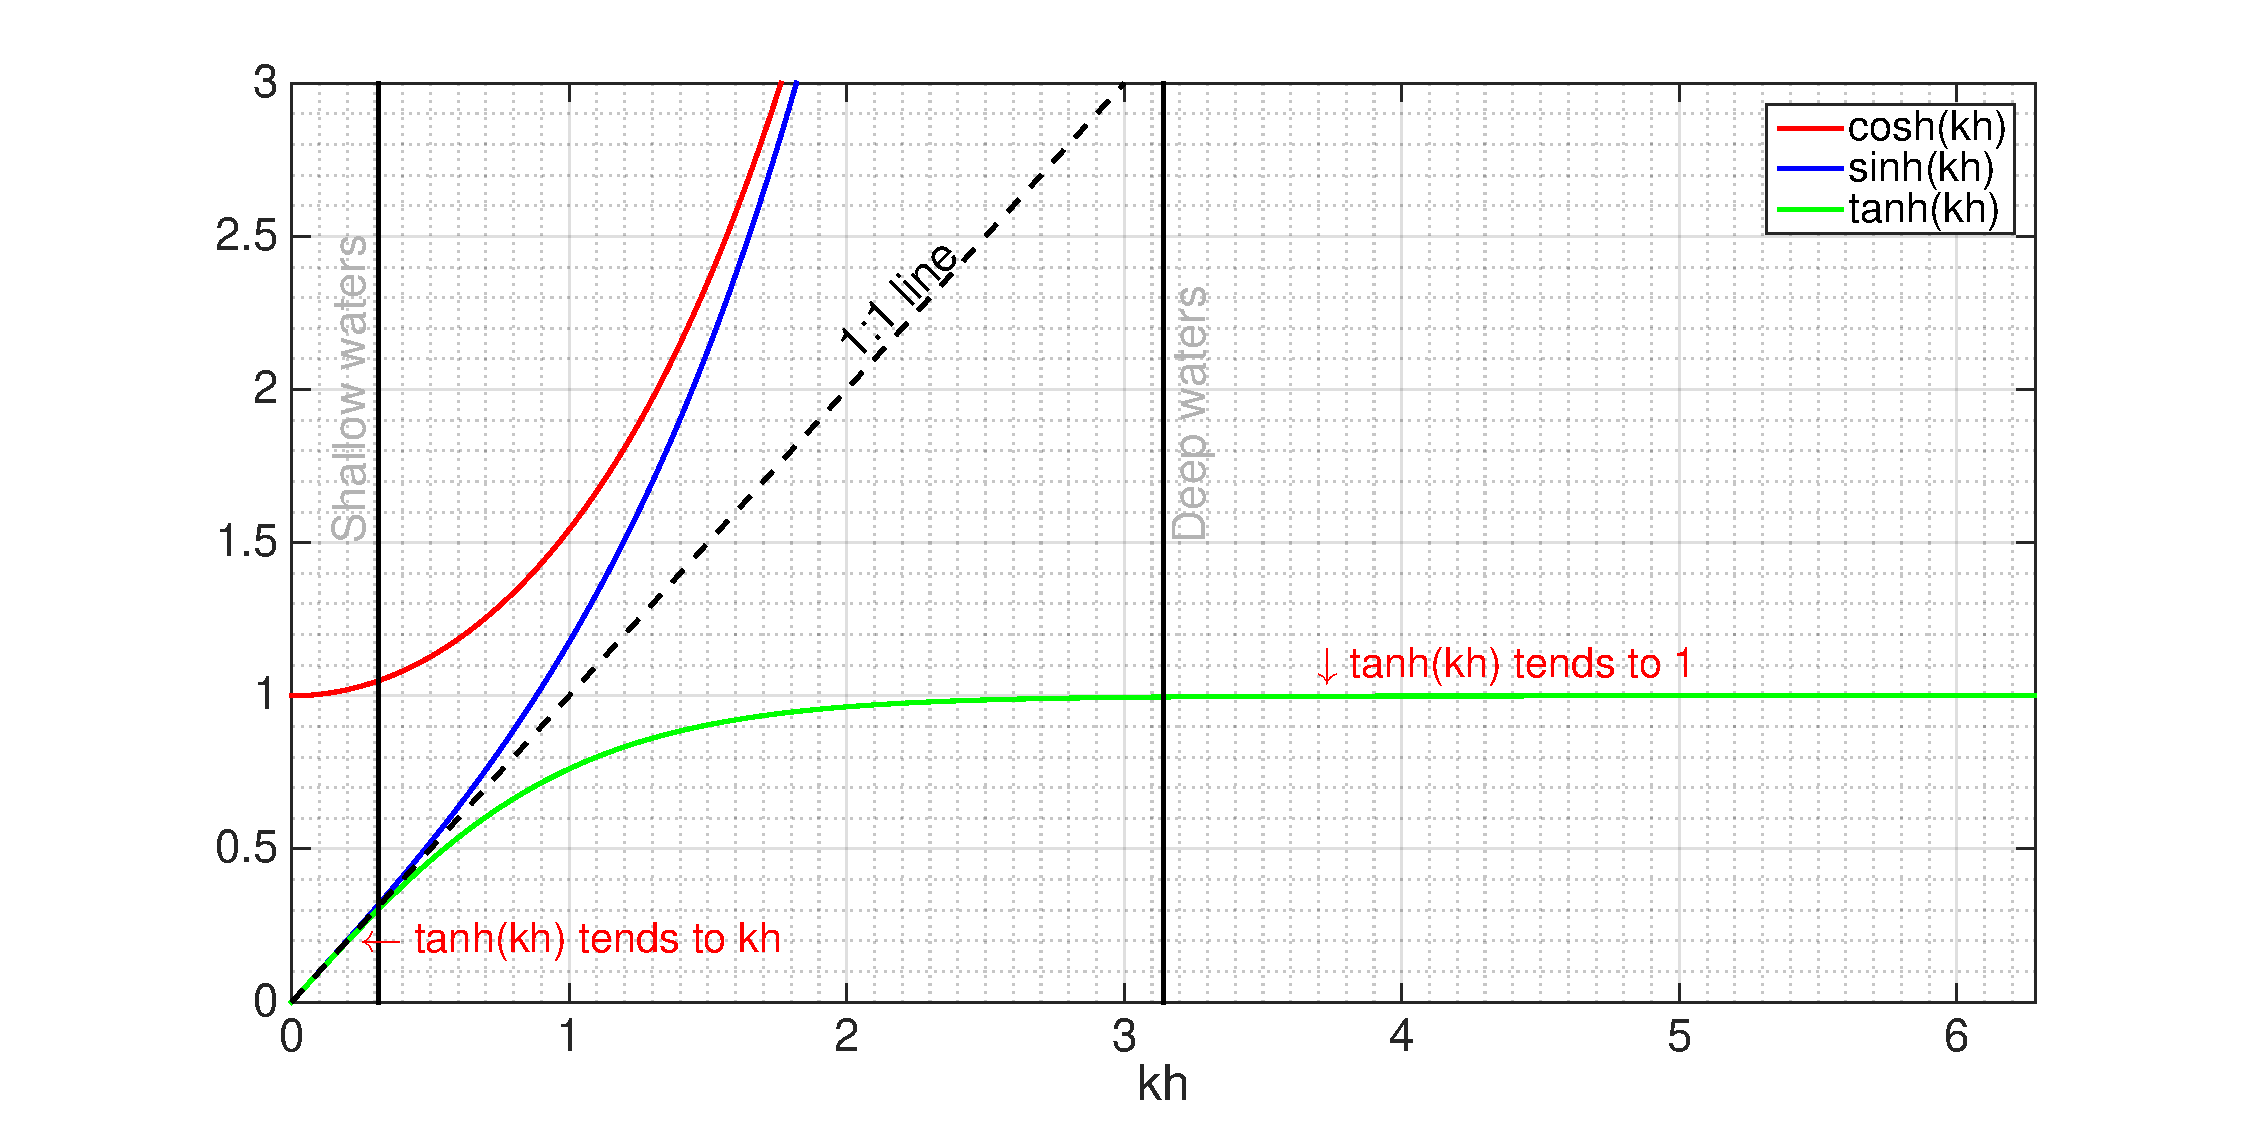
\includegraphics[width=\textwidth]{./SurfWaves_figs/Asymptotics.pdf} 
\caption{Asymptotic behaviour of the hyperbolic functions}\label{asympt}
\end{figure}
The previous treatment applies for any value of $kh$. However, for extremal values of this product, i.e. in the previously introduced classes of the \textbf{deep water} and \textbf{shallow water} the previous formulas are severely simplified. 
\subsubsection*{Deep water}
Referring to Figure \ref{asympt} the hyperbolic functions are clearly showing an asymptotic behaviour approaching $kh\rightarrow0$ and for $kh\rightarrow\infty$. The first approximation is the \textbf{Deep Water Asymptotic}, that is for $kh\rightarrow\infty$. Taking the limits for it is easy to prove that
\begin{align*}
\sinh\rbkt{kh}&\equiv\dfrac{e^{kh}-e^{-kh}}{2}\quad\overset{kh\rightarrow\infty}{\rightarrow}\quad\dfrac{1}{2}e^{kh}\\
\cosh\rbkt{kh}&\equiv\dfrac{e^{kh}+e^{-kh}}{2}\quad\overset{kh\rightarrow\infty}{\rightarrow}\quad\dfrac{1}{2}e^{kh}\\
\tanh\rbkt{kh}&\equiv\dfrac{e^{kh}-e^{-kh}}{e^{kh}+e^{-kh}}\quad\overset{kh\rightarrow\infty}{\rightarrow}\quad 1\\
\coth\rbkt{kh}&\equiv\dfrac{e^{kh}+e^{-kh}}{e^{kh}-e^{-kh}}\quad\overset{kh\rightarrow\infty}{\rightarrow}\quad 1
\end{align*}
that implies 
\begin{equation*}
G\equiv \dfrac{2kh}{\sinh\rbkt{2kh}}\quad\overset{kh\rightarrow\infty}{\rightarrow}\quad 0
\end{equation*}
and also
\begin{align*}
\dfrac{\cosh\sbkt{k\rbkt{z+h}}}{\sinh\rbkt{kh}}&\equiv \dfrac{e^{k\rbkt{z+h}}+e^{-k\rbkt{z+h}}}{e^{kh}-e^{-kh}}\quad\overset{kh\rightarrow\infty}{\rightarrow}\quad e^{kz}\\
\dfrac{\sinh\sbkt{k\rbkt{z+h}}}{\sinh\rbkt{kh}}&\equiv \dfrac{e^{k\rbkt{z+h}}-e^{-k\rbkt{z+h}}}{e^{kh}-e^{-kh}}\quad\overset{kh\rightarrow\infty}{\rightarrow}\quad e^{kz}\\
\dfrac{\cosh\sbkt{k\rbkt{z+h}}}{\cosh\rbkt{kh}}&\equiv \dfrac{e^{k\rbkt{z+h}}+e^{-k\rbkt{z+h}}}{e^{kh}+e^{-kh}}\quad\overset{kh\rightarrow\infty}{\rightarrow}\quad e^{kz}.
\end{align*}
With these simplifications the general formulas assumes a different shape. Denoting with the subscript $0$ the deep water condition
\begin{align}
k&=2\pi/L_{0}\\
\omega&=2\pi/T\\
c_{0}&=\sqrt{\dfrac{g}{k_{0}}}\\
c_{g0}&=\dfrac{c_{0}}{2}\\
u&=\dfrac{H_{0}\pi}{T}e^{k_{0}z}\cos\rbkt{\omega t -k_{0}x}\\
w&=-\dfrac{H_{0}\pi}{T}e^{k_{0}z}\sin\rbkt{\omega t -k_{0}x}\\
x&=\xi + \dfrac{H_{0}}{2}e^{k_{0}\zeta}\sin\rbkt{\omega t-k_{0}\xi}\\
z&=\zeta+\dfrac{H_{0}}{2}e^{k_{0}\zeta}\cos\rbkt{\omega t-k_{0}\xi}\\
p^{+}&=\rho g\dfrac{H_{0}}{2}e^{k_{0}z}\cos\rbkt{\omega t -k_{0}x}.
\end{align}
From this set of equation it can be seen that the particles are following circle-like paths, of which radius is a function of the depth but it exponentially decreases as $e^{k_{0}\zeta}$. 
\subsubsection*{Shallow water asymptotic}
The second asymptotic is the \textbf{Shallow Water Asymptotic}, that is taken as valid for $h/L<1/20$
\begin{align*}
\sinh\rbkt{kh}&\quad\overset{kh\rightarrow 0}{\rightarrow}\quad kh\\
\cosh\rbkt{kh}&\quad\overset{kh\rightarrow 0}{\rightarrow}\quad 1\\
\tanh\rbkt{kh}&\quad\overset{kh\rightarrow 0}{\rightarrow}\quad kh\\
\coth\rbkt{kh}&\quad\overset{kh\rightarrow 0}{\rightarrow}\quad \rbkt{kh}^{-1}
\end{align*}
that implies 
\begin{equation*}
G\equiv \dfrac{2kh}{\sinh\rbkt{2kh}}\quad\overset{kh\rightarrow 0}{\rightarrow}\quad 1
\end{equation*}
and also
\begin{align*}
\dfrac{\cosh\sbkt{k\rbkt{z+h}}}{\sinh\rbkt{kh}}&\quad\overset{kh\rightarrow 0}{\rightarrow}\quad \rbkt{kh}^{-1}\\
\dfrac{\sinh\sbkt{k\rbkt{z+h}}}{\sinh\rbkt{kh}}&\quad\overset{kh\rightarrow 0}{\rightarrow}\quad 1+\dfrac{z}{h}\\
\dfrac{\cosh\sbkt{k\rbkt{z+h}}}{\cosh\rbkt{kh}}&\quad\overset{kh\rightarrow 0}{\rightarrow}\quad 1.
\end{align*}
The general formulas thus becomes
\begin{align}
k&=\omega/\sqrt{gh}\\
L&=\sqrt{gh}T\\
c&=\sqrt{gh}\\
c_{g}&=c\\
u&=\dfrac{H}{2}\dfrac{c}{h}\cos\rbkt{\omega t -kx}\\
w&=-\dfrac{H}{2}\dfrac{ck}{h}\rbkt{h+z}\sin\rbkt{\omega t -kx}\\
x&=\xi + \dfrac{H}{2}\dfrac{L}{2\pi h}\sin\rbkt{\omega t-k\xi}\\
z&=\zeta+\dfrac{H}{2}\rbkt{1+\dfrac{z}{h}}\cos\rbkt{\omega t-k\xi}\\
p^{+}&=\rho g\dfrac{H}{2}\cos\rbkt{\omega t -kx}.
\end{align}
An important note on the shallow water asymptotic: the shallow water waves are not dispersive, that means that waves with different frequencies remains in the same wave packet.
\section{Wave Energy and dissipation processes}\label{Energy}
The wave energy will be purely mechanical, that means composed of a potential component and a kinetic one, where the potential energy originates from the displacement of the surface from a reference plane, while the kinetic energy arises from the wave particles velocity. The total energy is 
\begin{equation}
E_{T}=E_{p}+E_{k}.
\end{equation}
The potential energy can be evaluated from the mean-water level to the top of the wave as
\begin{align*}
E_{p}\rbkt{\theta}&=\int_{-h}^{\eta} \rho gz\,dz-\int_{-h}^{0}\rho gz \,dz=\int_{0}^{\eta}\rho gz \,dz\\
&=\rho g \left.\dfrac{z^{2}}{2}\right|^{\eta}_{0}=\dfrac{1}{2}\rho g\eta^{2}.
\end{align*}
Averaging this energy over the wave length, that is over $L$ (or $T$, since $L=cT$), the result is 
\begin{align*}
E_{p}&=\dfrac{1}{2L}\int_{0}^{L}\rho g \eta^{2}\,dx=\dfrac{\rho g}{2L}\int_{0}^{L} \eta^{2}\,dx=\dfrac{\rho g}{2L}\int_{0}^{L} \dfrac{H^{2}}{4}\cos^{2}\rbkt{\omega t-kx}\,dx\\
&\overset{\footnotemark}{=}\dfrac{1}{16}\rho g H^{2}.
\end{align*}\footnotetext{The integral is evaluated with the substitution
\begin{align*}
u&=\omega t -kx, \quad \left. u\right|_{x=0}=\omega t, \quad \left. u\right|_{x=L}=\omega t-kL=\omega t -2\pi\\
du&= -k\,dx
\end{align*}
that thus results in
\begin{align*}
\int_{0}^{L}\cos^{2}\rbkt{\omega t -kx}\,dx&=-\dfrac{1}{k}\int_{0}^{-2\pi}\cos^{2}\rbkt{u}\,du=-\dfrac{1}{k}\int_{0}^{-2\pi}\dfrac{1+\cos\rbkt{2u}}{2}\,du\\
&=-\dfrac{1}{k}\sbkt{\dfrac{u}{2}+\dfrac{\sin\rbkt{2u}}{4}}^{-2\pi}_{0}=\dfrac{\pi}{k}=\dfrac{L}{2}.
\end{align*}}
The potential energy is thus proportional to $H^{2}$ and hence always positive. The Kinetic energy has a more cumbersome computation. Starting from the specific energy
\begin{equation*}
e_{k}\rbkt{\theta}=\dfrac{1}{2}\rho\rbkt{u^{2}+w^{2}}=\dfrac{1}{2}\rho\rbkt{\dfrac{H\omega}{2\sinh\rbkt{kh}}}^{2}\rbkt{\cosh^{2}\sbkt{k\rbkt{z+h}}\cos^{2}\rbkt{\theta}+
\sinh^{2}\sbkt{k\rbkt{z+h}}\sin^{2}\rbkt{\theta}}
\end{equation*}
using the dispersion relation $\omega^{2}=gk\tanh\rbkt{kh}$ in the first parenthesis
\begin{equation*}
e_{k}\rbkt{\theta}=\dfrac{1}{4}\rho\rbkt{\dfrac{gkH^{2}}{2\sinh\rbkt{kh}\cosh\rbkt{kh}}}\rbkt{\cosh^{2}\sbkt{k\rbkt{z+h}}\cos^{2}\rbkt{\theta}+
\sinh^{2}\sbkt{k\rbkt{z+h}}\sin^{2}\rbkt{\theta}}
\end{equation*}
And furthermore, with the hyperbolic relations 
\begin{align*}
2\sinh\rbkt{\xi}\cosh\rbkt{\xi}&=\sinh\rbkt{2\xi}\\
\cosh^{2}\rbkt{\xi}&=1+\sinh^{2}\rbkt{\xi}
\end{align*}
and the classical trigonometric relation $\cos^{2}\rbkt{\xi}=1-\sin^{2}\rbkt{\xi}$ the energy can be rewritten as
\begin{equation}
e_{k}\rbkt{\theta}=\dfrac{\rho}{4}\rbkt{\dfrac{gH^{2}}{\sinh\rbkt{2kh}}}\rbkt{\cos^{2}\rbkt{\theta}+\sinh^{2}\sbkt{k\rbkt{z+h}}}.
\end{equation}
Integrating this relation over the depth
\begin{align*}
E_{k}\rbkt{\theta}&=\dfrac{\rho}{4}\rbkt{\dfrac{gH^{2}}{\sinh\rbkt{2kh}}}\sbkt{h\cos^{2}\rbkt{\theta}+\int_{-h}^{0}\sinh^{2}\sbkt{k\rbkt{z+h}}\,dz}\\
&=\dfrac{\rho}{4}\rbkt{\dfrac{gH^{2}}{\sinh\rbkt{2kh}}}\sbkt{h\cos^{2}\rbkt{\theta}+\int_{-h}^{0}\dfrac{1}{2}\rbkt{\cosh^{2}\sbkt{2k\rbkt{z+h}}-1}\,dz}\\
&=\dfrac{\rho}{4}\rbkt{\dfrac{gH^{2}}{\sinh\rbkt{2kh}}}\sbkt{h\rbkt{\cos^{2}\rbkt{\theta}-\dfrac{1}{2}}+\dfrac{1}{4k}\sinh^{2}\sbkt{2k\rbkt{z+h}}_{-h}^{0}}\\
&=\dfrac{\rho gH^{2}}{4\sinh\rbkt{2kh}}\sbkt{h\rbkt{\cos^{2}\rbkt{\theta}-\dfrac{1}{2}}+\dfrac{\sinh^{2}\rbkt{2kh}}{4k}}\\
&=\dfrac{1}{16}\rho gH^{2} + \dfrac{1}{8}\rho gH \dfrac{2kh}{\sinh\rbkt{2kh}}\sbkt{\cos^{2}\rbkt{\theta}-\dfrac{1}{2}}
\end{align*}
and again integrating over the wave length $L$ the kinetic energy is found as
\begin{equation}
E_{k}=\dfrac{1}{16}\rho g H^{2}.
\end{equation}
Finally, the total mechanical energy can be computed and gives
\begin{equation}
E=\dfrac{1}{8}\rho g H^{2}.
\end{equation}
\subsection{Shoaling and Refraction}\label{RefractionShoaling}
Shoaling refers to areas where the water depth is not constant. but varies so slowly that the bottom slope is small everywhere. Two fundamental assumptions are that the slope is so small that no reflection occurs for short periodic waves and that the slope is so small that it does not affect the wave. There are two possibilities of behaviour for the wave approaching the land, it can be seen the simple shoaling phenomena, when the water waves approaches the shore perpendicularly, or there can be a refraction effect, where the wave have an incident angle $\alpha$ with respect to the shoreline and consequently it changes the path due to the effect of the that different depths under the wave front. In this latter case, the analogy with optics will be crucial. 
\subsubsection*{Simple shoaling}
Supposing that no dissipation occurs during the shoaling process, that is the approaching of a wave towards the shore among a gently sloped bottom, the energy flux in between two different vertical sections $1$ and $2$ is preserved, that means
\begin{equation*}
E_{f,1}=E_{f,2},
\end{equation*}
but since
\begin{equation*}
E_{f}=H^{2}c\rbkt{1+2G}, \qquad G=\dfrac{2kh}{\sinh\rbkt{2kh}}
\end{equation*}
the former conservation statement can be rewritten as
\begin{equation*}
H_{1}^{2}c_{1}\rbkt{1+2G_{1}}=H_{2}^{2}c_{2}\rbkt{1+2G_{2}}.
\end{equation*}
Recalling that $c=c_{0}\tanh\rbkt{kh}$ the height $H_{2}$ can be rewritten as
\begin{equation*}
H_{2}=H_{1}\rbkt{\dfrac{\tanh\rbkt{k_{1}h_{1}}}{\tanh\rbkt{k_{2}h_{2}}}\dfrac{1+G_{1}}{1+G_{2}}}^{1/2}
\end{equation*}
that results in a relation to evaluate $H_{2}$ when $H_{1}$ and $h_{1}$ are known. Often, these two will correspond to deep water condition, thus the equation can be rewritten as
\begin{equation}
H=H_{0}\rbkt{\tanh\rbkt{kh}\rbkt{1+G}}^{-1/2}
\end{equation}
and so introduce the \textbf{shoaling coefficient}
\begin{equation}
K_{s}=\rbkt{\tanh\rbkt{kh}\rbkt{1+G}}^{-1/2}.
\end{equation}
The functional form of $K_{s}$ presents a minimum, attained at $1/2\pi$, where $K_{s}=0.93$. This minimum is where $c_{g}$ is maximum. This maximum-minimum symmetry is obvious when thinking that when the celerity is higher the water depth will be small in order to conserve energy (and mass). 
\subsubsection*{Refraction shoaling}
As the wave approaches the shore at an angle $\alpha$ the wave front will show different behaviours due to the differences in the underlying bathymetry. As a result, the front will move with different velocities in its different parts, slowing as it approaches the shore. This process will make sure that the wave will be always close to being parallel to the shoreline. Indeed, as a wave propagates towards the shore, the wave length decreases as the depth decreases, since
\begin{equation*}
c^{2}=\dfrac{g}{k}\tanh\rbkt{kh},\quad c=\dfrac{\omega}{k}
\end{equation*}
and hence 
\begin{equation*}
\omega^{2}=gk\tanh\rbkt{kh} \quad \rightarrow \quad \dfrac{1}{k}=\dfrac{g}{\omega}\tanh\rbkt{kh} 
\end{equation*}
and thus
\begin{equation}
L=\dfrac{g}{2\pi}T^{2}\tanh\rbkt{kh}.
\end{equation}
Consequently, also $c$ becomes smaller. The result is that the wave refracts, changing gradually his approaching angle. A simplified approach is that of the optic similarity. Two waves at to sides of the bathymetry contour (i.e. a change in the depth) moves with the same period $T$, but different celerity and length, so
\begin{equation*}
T^{sx}=T^{dx} \quad \rightarrow \quad \dfrac{L^{sx}}{c_{1}}=\dfrac{L^{dx}}{c_{2}}
\end{equation*}
so that
\begin{equation*}
\dfrac{\lambda\sin\theta_{1}}{c_{1}}=\dfrac{\lambda\sin\theta_{2}}{c_{2}}
\end{equation*}
which means
\begin{equation}
\dfrac{\lambda\sin\theta}{c}=const,
\end{equation}
also known as Snell's Law. This refraction will have an important role in evaluating the height of a shoaling wave, as thanks to the conservation of energy $E_{1}c_{g1}L_{1}=E_{2}c_{g2}L_{2}$ it can be found that
\begin{equation}
\dfrac{H_{1}}{H_{2}}=\sqrt{\dfrac{c_{g1}}{c_{g2}}}\sqrt{\dfrac{\cos\theta_{1}}{\cos\theta_{2}}}
\end{equation}
or also
\begin{equation}
H=H_{0}K_{s}K_{r}, \quad K_{s}=\sqrt{\dfrac{c_{g}}{c_{g0}}} \quad K_{r}=\sqrt{\dfrac{\cos\theta}{\cos\theta_{0}}}
\end{equation}
in analogy with the simple shoaling case.
\subsection{Breaking}\label{Breaking}
In deep water, waves breaks because of an excessive energy input coming from the wind. Usually, when the wind speed is more than a certain value ($1m/s$) and wind waves starts to develop, if the celerity $\mathbf{c}$ of the wave resembles the wind speed the waves starts to develop the so called \textit{white caps}, a dissipation process that dissipates the energy of the \textit{fully arisen sea} (or FAS). This phenomena happens when the wave steepness $H/L$ reaches the critical value of
\begin{equation}
\dfrac{H_{0}}{L_{0}}\approx 0.17 \qquad \text{(Mitchell's criteria)}.
\end{equation}
In shallow water waves continue to shoal until they become so large that they become unstable and break. The breaking wave characteristic can be correlated to the \textbf{surf similarity parameter} $\xi$ (or \textbf{Iribarren Parameter})
\begin{equation}
\xi = \tan\beta/\sqrt{H_{0}/L_{0}}.
\end{equation}
This parameter describes the type of breaking that can happen, depending on the beach slope $\beta$ and the deep water steepness $H_{0}/L_{0}$. With the surf similarity parameter the breaker index $\kappa$ can be evaluated as 
\begin{equation}
\kappa=\xi^{0.17}+0.08
\end{equation}
which is used to linearly relate the breaking height with the breaking depth
\begin{equation}
H_{b}=\kappa h_{b}.
\end{equation}
The minimum value of $\kappa$ is $\kappa=0.78$ for constant depth water, and is called Munk relation.
\begin{figure}
\centering
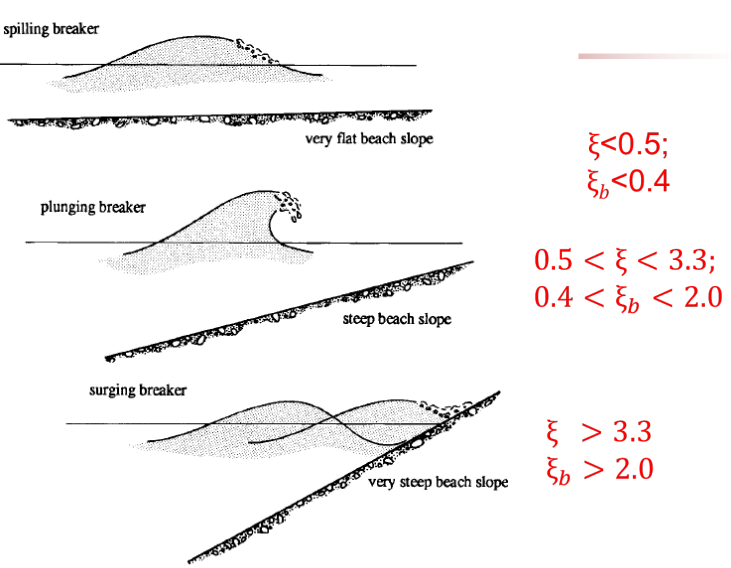
\includegraphics[width=0.5\textwidth]{./SurfWaves_figs/breaker_types.png} 
\caption{Different Iribarren Parameter value for different types of breaking}
\end{figure}
\subsubsection{Dean Dalrymple model}
\textbf{Facts} \\ \\
- if the wave height $H > 0.78 h$ ($h$ is the water depth) then the wave breakes and losses energy until $H = 40 \% ~ h$\\ \\ 
- otherwise, if the wave height $H \le 0.78 h$, it doesn't break, it goes towards the shore undisturbed, even if $H > H_{st} = 40 \% h$\\ \\
\textbf{Formula} \\ \\
Water depth: $h$ \\ \\
Generic Wave Height: $H$ \\ \\
Stable Wave Height: $H_{st}(h) = \Gamma ~ h = 0.4 ~ h$ \\ \\ 
Wave Energy: $E = \rho ~ g ~ \frac{H^2} 8$ \\ \\
Stable Wave Energy: $E_{st} = \rho ~ g ~ \frac{H_{st}^2} 8 = \rho ~ g ~ \frac{ \Gamma^2  h^2} 8$ \\ \\
Group velocity along $\hat{x}$ in shallow waters: $c_g   \approx  \sqrt{g h}$ \\ \\
Total derivative of wave energy with dissipation: $\partial_t E + \partial_x(E ~ c_g) = D$   \\ \\ 
Steady conditions: ($\partial_t E = 0$) imply that
$\partial_x(E ~ c_g) = D$ \\ \\ 
Dissipation rate according to Dean-Dalrymple model:
\\
\begin{center}
D =  $\begin{bmatrix}
	\frac k h ( E ~ c_g - E_{st} ~ c_g) & , H > H_{br}\\
	0 & H \le H_{br}\\
  \end{bmatrix}$
\end{center}
where $k = 0.15$. So in case $ H > H_{br}$ the energy equation becomes:
\[
	\partial_x(E ~ c_g) = \frac k h ( E ~ c_g - E_{st} ~ c_g)
\]
\[
	\partial_x(\frac{H^2 \rho g} 8 ~ \sqrt{g h}) 
		= \frac k h ( \frac{H^2 \rho g} 8 ~ \sqrt{g h} 
				- \frac{H_{st}^2 \rho g} 8 ~ \sqrt{g h})
\]
\[
	\partial_x( H^2 ~ \sqrt{h}) 
		= \frac k h ( H^2 ~ \sqrt{h} 
				- H_{st}^2 ~ \sqrt{h})
\]
\[
	\partial_x( H^2 ~ \sqrt{h}) 
		= \frac k h ( H^2 ~ \sqrt{h} 
				- \Gamma^2 ~ h^2 ~ \sqrt{h})
\]
\[
	\partial_x( H^2 ~ \sqrt{h}) 
		= \frac {0.15} h ( H^2 ~ \sqrt{h} 
				- 0.4^2 ~ h^2 ~ \sqrt{h})
\]
\subsection{Radiation Stress}\label{Rad_stress}
\section{Random waves}\label{Rand_sea}
The treatment explained in the previous sections deals lies its foundation on the assumption of sinusoidal waves. This kind of waves are observable only in laboratory, in the natural environment waves are never sinusoidal. Sea waves are characterised by a great amount of randomness, it is impossible to describe the sea level at a certain ocean location deterministically. In the engineering practice, statistical parameters are evaluated in order to get some parameters to use in the evaluation of the physical properties of the wave. In other words it is possible to find and study the distributions which describe the statistical behaviour of wave height,period,frequency and also direction of the incoming waves at a particular location. A starting point is the \textit{zero-upcrossing method} (or equivalently the \textit{zero-downcrossing method}). This method uses the recordings of the water level over a period of time. The mean water level is deduced from the surface record and defined as the zero line. Then, a research of the first instant in which the line crosses the zero line upwards (for the zero-upcrossing or equivalently downwards for the zero-downcrossing) and, once found it is settled as the starting point for a single wave. Following the ups and downs of the wave the endpoint is chosen as the next zero-upcrossing (equivalently, zero down-crossing) point. The endpoint of wave $i$ defines of course the starting point of the wave $i+1$. The vertical distance between the highest point and the lowest point is defined as the \textbf{wave height}. After applying this method over a recording on the water surface, a list of individual waves is produced. Over this list, rearranged to be decreasing in terms of wave height, some statistically significant representative waves can be defined:
\begin{itemize}
\item \textbf{Highest wave}: $H_{max}, T_{max}$. This wave is the highest one among all the simple waves of the time series;
\item \textbf{Highest one-tenth wave}: $H_{1/10}, T_{1/10}$. These two values represent the mean of the highest one-tenth of the entire number of waves;
\item \textbf{Significant wave, or Highest one-third wave}: $H_{1/3}, T_{1/3}$. These two values represent the averaged highest one-third of the record;
\item \textbf{Mean wave}: $\bar{H}, \bar{T}$. These two values represent the mean values of the entire waves series.
\end{itemize}
Among the previously introduced parameters, the significant wave is the most used.



\subsubsection*{Questions}
\begin{itemize}
\item How can we describe the wave kinematic through the Airy theory (velocity, celerity)? What is the dispersion relationship, what is the general expression and what are the asymptotic forms? See Section \ref{Airy}
\item Define the potential and derive the kinetic properties of the waves. See Section \ref{solution}
\item Find the dispersion relationship and discuss the shallow and deep approximations
\item What is the wave height and what is the significant wave height. See Section \ref{Rand_sea}
\item What is the concept of wave energy and what formula describes it? What are the group and wave celerity?. %See Section \ref{Energy}
\item Explain Snell’s law and wave refraction. See Section \ref{RefractionShoaling}
\item Explain wave shoaling with formula. See Section \ref{RefractionShoaling}
\item Explain the breaking process and the model used to describe it. See Section \ref{Breaking}
\item Describe the Radiation. See Stress. Section \ref{Rad_stress}
\item Explain wave setup and wave runup. See Section \ref{Rad_stress}
\item Discuss the irregular nature of waves: how can we characterize its randomness? See Section \ref{Rand_sea}
\end{itemize}
\chapter{Geophysical fluid dynamics}
\section{Equations of motions}\label{motionEQ}
Whenever a fluid undergoes non uniform translation and rotation the effects of the non inertial reference frame appear. In atmospheric and oceanic sciences, or simply in geophysical fluid dynamics, the effects of the Earth's rotation plays an important role, thus the Earth fixed reference frame must be treated as a the rotating frame which is. Considering a reference frame $O'1'2'3'$ that is located in a position $\mathbf{X}\rbkt{t}$ with respect to a fixed reference frame $O123$. Suppose that the non inertial reference is moving with velocity
\begin{equation*}
\dfrac{d}{dt}\mathbf{X}\rbkt{t}=\mathbf{U}\rbkt{t}
\end{equation*}
and rotating with angular frequency $\bs{\Omega}\rbkt{t}$. Considering a fluid particle located at a point $P$ in space, this point can be localized in the inertial reference frame $O123$ with the vector $\mathbf{x}=\rbkt{x_{1},x_{2},x_{3}}$ and in the non inertial reference $O'1'2'3'$ with the vector $\mathbf{x}'=\rbkt{x_{1}',x_{2}',x_{3}'}$, where these two distances are related by the relation
\begin{equation*}
\mathbf{x}\rbkt{t}=\mathbf{X}\rbkt{t}+\mathbf{x}'\rbkt{t}.
\end{equation*}
Differentiating in time (and dropping the notation of the temporal dependence) the velocity can be computed as
\begin{align*}
\mathbf{u}&=\dfrac{d\mathbf{X}}{dt}+\dfrac{d\mathbf{x}'}{dt}=\mathbf{U}+\dfrac{d}{dt}\rbkt{x_{1}'\mathbf{e}_{1}'+x_{2}'\mathbf{e}_{2}'+x_{3}'\mathbf{e}_{3}'}\\
&=\mathbf{U}+\dfrac{dx_{1}'}{dt}\mathbf{e}_{1}'+\dfrac{dx_{2}'}{dt}\mathbf{e}_{2}'+\dfrac{dx_{3}'}{dt}\mathbf{e}_{3}'+x_{1}'\dfrac{d\mathbf{e}_{1}'}{dt}+x_{2}'\dfrac{d\mathbf{e}_{2}'}{dt}+x_{3}'\dfrac{d\mathbf{e}_{3}'}{dt}\\
&=\mathbf{U}+\mathbf{u}'+\bs{\Omega}\times\mathbf{x}'
\end{align*}
while the acceleration follows after another temporal differentiation:
\begin{align*}
\mathbf{a}&=\dfrac{d\mathbf{U}}{dt}+\dfrac{d\mathbf{u}'}{dt}+\dfrac{d}{dt}\rbkt{\bs{\Omega}\times\mathbf{x}'}=\mathbf{A}+\dfrac{d\mathbf{u}'}{dt}+\dfrac{d}{dt}\rbkt{\bs{\Omega}\times\mathbf{x}'}\\
&=\mathbf{A}+\dfrac{d}{dt}\rbkt{u_{1}',u_{2}',u_{3}'}\rbkt{\mathbf{e}_{1}',\mathbf{e}_{2}',\mathbf{e}_{3}'}^{T}+\dfrac{d}{dt}\rbkt{\bs{\Omega}\times\mathbf{x}'}\\
&=\mathbf{A}+\dfrac{du_{1}'}{dt}\mathbf{e}_{1}'+\dfrac{du_{2}'}{dt}\mathbf{e}_{2}'+\dfrac{du_{3}'}{dt}\mathbf{e}_{3}'+u_{1}'\dfrac{d\mathbf{e}_{1}'}{dt}+u_{2}'\dfrac{d\mathbf{e}_{2}'}{dt}+u_{3}'\dfrac{d\mathbf{e}_{3}'}{dt}
+\dfrac{d\bs{\Omega}}{dt}\times\mathbf{x}'+\bs{\Omega}\times\dfrac{d\mathbf{x}'}{dt}\\
&=\mathbf{A}+\mathbf{a}'+\bs{\Omega}\times\mathbf{u}'+\dfrac{d\bs{\Omega}}{dt}\times\mathbf{x}'+\bs{\Omega}\times
\rbkt{\mathbf{u}'+\bs{\Omega}\times\mathbf{x}'}\\
&=\mathbf{A}+\mathbf{a}'+2\bs{\Omega}\times\mathbf{u}'+\dfrac{d\bs{\Omega}}{dt}\times\mathbf{x}'+\bs{\Omega}\times\bs{\Omega}\times\mathbf{x}'.
\end{align*}
In this expression $\mathbf{A}$ is the acceleration of the reference $O'1'2'3'$ with respect to the reference $O123$, $\mathbf{a}'$ is the acceleration of $P$ with respect to the non inertial reference $O'1'2'3'$. The term $2\bs{\Omega}\times\mathbf{u}'$ is the \textbf{Coriolis acceleration}, of which effects will be the main topic of this chapter. The term $d\bs{\Omega}/dt\times\mathbf{x}'$ is the acceleration caused by the angular acceleration of the reference frame, while $\bs{\Omega}\times\bs{\Omega}\times\mathbf{x}'$ is the centrifugal acceleration. Using the material derivative symbol for the acceleration, the previous definition can be rewritten as
\begin{equation*}
\rbkt{\dfrac{D\mathbf{u}}{Dt}}_{O123}=\rbkt{\dfrac{D\mathbf{u}'}{Dt}}_{O'1'2'3'}+\dfrac{d\mathbf{U}}{dt}+2\bs{\Omega}\times\mathbf{u}'+\dfrac{d\bs{\Omega}}{dt}\times\mathbf{x}'+\bs{\Omega}\times\bs{\Omega}\times\mathbf{x}'
\end{equation*}
and finally the Navier-Stokes equations in a non inertial reference frame can be stated as
\begin{equation}
\rho\rbkt{\dfrac{D'\mathbf{u}'}{Dt}}=-\nabla' p +\rho\rbkt{\mathbf{g}-\dfrac{d'\mathbf{U}}{dt}-2\bs{\Omega}\times\mathbf{u}'-\dfrac{d'\bs{\Omega}}{dt}\times\mathbf{x}'-\bs{\Omega}\times\bs{\Omega}\times\mathbf{x}'}+\mu\Delta'\mathbf{u}'
\end{equation}
where the apexes refers to the fact that this equation settles in the reference $O'1'2'3'$ and from now on will be dropped. The last step is to specialize this set of equations for the dynamic of fluids over the Earth, that is specifying the Geophysical Fluid Dynamics equations of motion. This will be done by dropping those terms of which influence is negligible if not zero. The acceleration and the angular acceleration of the earth, $d\mathbf{U}/dt$ and $d\bs{\Omega}/dt\times\mathbf{x}'$, can be dropped without any problem. The centrifugal acceleration $\bs{\Omega}\times\bs{\Omega}\times\mathbf{x}'$ can be incorporated in the gravity term $g$ by noticing that, in a cylindrical set of coordinates $\rbkt{R,\varphi,z}$ with the angular rotation $\bs{\Omega}=\rbkt{0,0,\Omega}$ this term can be expressed as $\bs{\Omega}\times\bs{\Omega}\times\mathbf{x}'=+\Omega^{2}R\mathbf{e}_{R}$ and thus the \textbf{effective gravity} can be defined as $\mathbf{g}=\mathbf{g_{n}}+\Omega^{2}R\mathbf{e}_{R}$. The GFD equations of motion can finally be written as
\begin{equation}\label{GFmotion}
\rho\rbkt{\dfrac{D\mathbf{u}}{Dt}+2\bs{\Omega}\times\mathbf{u}}=-\nabla p +\rho\mathbf{g}+\mu\Delta\mathbf{u}.
\end{equation}
Often geophysical flows can be treated with the further assumption of negligibility of density variations. This assumption is called \textbf{Boussinesq Approximation} and states that the density variations can be neglected except when multiplied by $g$. Taking a reference value $\rho_{s}$ for the density and dividing the previous equation the result is
\begin{equation*}
\dfrac{\rho}{\rho_{s}}\rbkt{\dfrac{D\mathbf{u}}{Dt}+2\bs{\Omega}\times\mathbf{u}}=-\dfrac{1}{\rho_{s}}\nabla p +\dfrac{\rho}{\rho_{s}}\mathbf{g}+\dfrac{\mu}{\rho_{s}}\Delta\mathbf{u}.
\end{equation*}
and so when the density variations $\rho/\rho_{s}\cong1$ and $\mu/\rho_{s}\cong\nu$ the equations of motion are
\begin{equation}
\dfrac{D\mathbf{u}}{Dt}+2\bs{\Omega}\times\mathbf{u}=-\dfrac{1}{\rho_{s}}\nabla p +\dfrac{\rho}{\rho_{s}}\mathbf{g}+\nu\Delta\mathbf{u}.
\end{equation}
Another consequence of the Boussinesq approximation is that the mass conservation statement 
\begin{equation*}
\dfrac{\partial\rho}{\partial t}+\nabla\cdot\rbkt{\rho\mathbf{u}}=0
\end{equation*}
thanks to this neglection of the variation in the density can be substituted by its incompressible version 
\begin{equation}
\nabla\cdot\mathbf{u}=0.
\end{equation}
Furthermore, the requirement of constant density $D\rho/Dt=0$ is made. The equations of motion for a geophysical problem can be summarized as
\begin{align}
\dfrac{D\mathbf{u}}{Dt}+2\bs{\Omega}\times\mathbf{u}&=-\dfrac{1}{\rho_{s}}\nabla p +\dfrac{\rho}{\rho_{s}}\mathbf{g}+\mathbf{F}\\
\nabla\cdot\mathbf{u}&=0\\
\dfrac{D\rho}{Dt}&=0
\end{align}
where the frictional forces have been substituted with the vector $\mathbf{F}$. With the \textbf{eddy viscosity assumption} the vector $\mathbf{F}$ can be rewritten as
\begin{align*}
F_{x}&=\dfrac{\partial\tau_{xx}}{\partial x}+\dfrac{\partial\tau_{xy}}{\partial x}+\dfrac{\partial\tau_{xz}}{\partial x}=\nu_{H}\rbkt{\dfrac{\partial^{2} u}{\partial x^{2}}+\dfrac{\partial^{2} u}{\partial y^{2}}}+\nu_{V}\rbkt{\dfrac{\partial^{2} u}{\partial z^{2}}}\\
F_{y}&=\dfrac{\partial\tau_{yx}}{\partial x}+\dfrac{\partial\tau_{yy}}{\partial x}+\dfrac{\partial\tau_{yz}}{\partial x}=\nu_{H}\rbkt{\dfrac{\partial^{2} v}{\partial x^{2}}+\dfrac{\partial^{2} v}{\partial y^{2}}}+\nu_{V}\rbkt{\dfrac{\partial^{2} v}{\partial z^{2}}}\\
F_{z}&=\dfrac{\partial\tau_{zx}}{\partial x}+\dfrac{\partial\tau_{zy}}{\partial x}+\dfrac{\partial\tau_{zz}}{\partial x}=\nu_{H}\rbkt{\dfrac{\partial^{2} w}{\partial x^{2}}+\dfrac{\partial^{2} w}{\partial y^{2}}}+\nu_{V}\rbkt{\dfrac{\partial^{2} w}{\partial z^{2}}}.
\end{align*}
\subsubsection*{Tangent plane approximation}
Theoretically, geophysical flow problems should be solved in a spherical polar reference system. However, a comparison between the vertical and horizontal scale suggests a different approach. As the scales of this kind of motion are on the order of 5 or 15 km in the vertical direction but on the order of hundreds or even thousands of kilometres, the trajectories can be considered nearly horizontal, as $\abs{u},\abs{v}\gg\abs{w}$ and most of geophysical flows occur in thin layers. Starting from this analysis it can be introduced a \textbf{local cartesian system on a tangent plane}. This cartesian reference is characterized by a coordinate $x$ increasing \textit{westward}, a coordinate $y$ increasing \textit{northward} and $z$ increasing \textit{upward}. With this tangent plane the Coriolis acceleration parameter can be evaluated. Denoting with $\theta$ the geographic latitude, the rotation vector $\bs{\Omega}$ in the tangent plane reference is 
\begin{equation}
\bs{\Omega}=\rbkt{\Omega_{x},\Omega_{y},\Omega_{z}}=\rbkt{0,\Omega\cos\theta,\Omega\sin\theta}
\end{equation}
where $\Omega\equiv\abs{\bs{\Omega}}=2\pi/86400s=7.27\times 10^{-5}\text{rad/s}$ is the earth rotation rate. The vector product
\begin{equation*}
2\bs{\Omega}\times\mathbf{u}=\left|\begin{array}{ccc}
\mathbf{e}_{x}&\mathbf{e}_{y}&\mathbf{e}_{x}\\
0&2\Omega\cos\theta&2\Omega\sin\theta\\
u&v&w
\end{array}\right|=
2\Omega\sbkt{\mathbf{e}_{x}\rbkt{w\cos\theta-v\sin\theta}+\mathbf{e}_{y}u\sin\theta-\mathbf{e}_{z}u\cos\theta}.
\end{equation*}
Away from the equator, where $\theta=0$, the thin-layer approximation $\abs{w}\ll\abs{v}$ allow $w\cos\theta$ to be ignored, so the components of the Coriolis acceleration are
\begin{equation*}
2\bs{\Omega}\times\mathbf{u}=\rbkt{-2\Omega v\sin\theta,2\Omega u\sin\theta,-2\Omega u\cos\theta}
\end{equation*}
and it can be written in the usual form as
\begin{equation}
2\bs{\Omega}\times\mathbf{u}=\rbkt{fv,fu,-2\Omega u\cos\theta}
\end{equation}
having introduced the \textbf{Coriolis parameter} $f=2\Omega\sin\theta$, called also \textit{planetary vorticity}, as it is twice the earth rotation rate. Moreover, the vertical component of the Coriolis acceleration, $-2\Omega u\cos\theta$ is negligible with respect to the other components of the vertical equation of motion (namely the pressure variation and the gravitational effect).
\subsubsection*{Pressure and density perturbations}
The pressure and the density can be regarded in the equations as pressure and density perturbations from a reference distribution \textit{at rest}. This is possible by separating the vertical distribution at rest as
\begin{equation}\label{perturbations}
\rho\rbkt{t,\mathbf{x}}=\bar{\rho}\rbkt{z}+\rho'\rbkt{t,\mathbf{x}}, \qquad p\rbkt{t,\mathbf{x}}=\bar{p}\rbkt{z}+p\rbkt{t,\mathbf{x}}
\end{equation}
where the static distributions $\bar{\rho}\rbkt{z}$ and $\bar{p}\rbkt{z}$ follows the hydrostatic law
\begin{equation}
\dfrac{dp}{dz}=-\rho g.
\end{equation}
The gravitational and pressure term in the equation of motion can be evaluated as
\begin{align*}
\nabla p +\rho g \mathbf{e}_{z}&=\nabla\rbkt{p+p'}+g\rbkt{\rho+\rho'}\mathbf{e_{z}}=\sbkt{\dfrac{d\bar{p}}{dz}+\rho g}\mathbf{e}_{z}+\nabla p' +g\rho'\mathbf{e}_{z}=\\
&=\nabla p' + g\rho' \mathbf{e}_{z}.
\end{align*}
\subsubsection*{Equation of motions}
Finally, the equations of motion can be written completely as:
\begin{align}
&\dfrac{Du}{Dt}-fv=-\dfrac{1}{\rho_{s}}\dfrac{\partial p'}{\partial x}+\nu_{H}\rbkt{\dfrac{\partial^{2} u}{\partial x^{2}}+\dfrac{\partial^{2} u}{\partial y^{2}}}+\nu_{V}\rbkt{\dfrac{\partial^{2} u}{\partial z^{2}}}\\
&\dfrac{Dv}{Dt}-fu=-\dfrac{1}{\rho_{s}}\dfrac{\partial p'}{\partial y}+\nu_{H}\rbkt{\dfrac{\partial^{2} v}{\partial x^{2}}+\dfrac{\partial^{2} v}{\partial y^{2}}}+\nu_{V}\rbkt{\dfrac{\partial^{2} v}{\partial z^{2}}}\\
&\dfrac{Dw}{Dt}=-\dfrac{1}{\rho_{s}}\dfrac{\partial p'}{\partial z}-\dfrac{g\rho'}{\rho_{s}}+\nu_{H}\rbkt{\dfrac{\partial^{2} w}{\partial x^{2}}+\dfrac{\partial^{2} w}{\partial y^{2}}}+\nu_{V}\rbkt{\dfrac{\partial^{2} w}{\partial z^{2}}}.
\end{align}
\subsubsection*{$f$-plane and $\beta$-plane models}
\section{Geostrophic Flow}
Away from boundaries, in a large-scale quasi-steady motion in the atmosphere or the ocean, a good approximation of the equation of motions is given by the \textbf{geostrophic balance}, where the Coriolis acceleration matches the horizontal pressure gradient acceleration
\begin{align*}
-fv&=-\dfrac{1}{\rho_{s}}\dfrac{\partial p}{\partial x}\\
fu&=-\dfrac{1}{\rho_{s}}\dfrac{\partial p}{\partial y}.
\end{align*}
Attention must be put on the absence of the apexes, as indeed differentiating $\eqref{perturbations}$ in $x$ or $y$ the equalities $\partial p/\partial x = \partial p'/\partial x $ and $\partial p/\partial y = \partial p'/\partial y $ are obtained. These equations have been obtained dropping the non linear term in the original geophysical equations of motion. This is possible if the \textbf{Rossby number} $\Rossby$ is small enough. The Rossby number compares the intensity of the non-linear acceleration and the Coriolis acceleration in terms of significative scales $U$ and $L$ characterizing the motion (velocity and length scale), and it can be expressed as
\begin{equation}
\Rossby=\dfrac{\text{Non-linear acceleration}}{\text{Coriolis acceleration}}\sim\dfrac{U^{2}/L}{fU}=\dfrac{U}{fL}.
\end{equation}
This parameter in the atmosphere is usually less than $0.1$, as $U\sim10m/s$, $f\sim10^{-4}$ and $L=1000km$, while in the ocean can be even smaller as the velocity is smaller. A \textit{Geostrophic Wind} is an atmospherical flow for which the Geostrophic Balance holds. In such a system the velocity distribution can be determined from pressure measurements. Finally it is straightforward to prove that the flow is perpendicular to the pressure gradient:
\begin{equation}
\rbkt{u\mathbf{e}_{x}  +v\mathbf{e}_{y} } \cdot \nabla p = \dfrac{1}{f\rho_s}\rbkt{-\mathbf{e}_{x}\dfrac{\partial p}{\partial y}  +\mathbf{e}_{y}\dfrac{\partial p}{\partial x} }
\rbkt{\mathbf{e}_{x}\dfrac{\partial p}{\partial x}  +\mathbf{e}_{y}\dfrac{\partial p}{\partial y} }=0
\end{equation}
so the \textbf{flow is along the line of costant pressure}, a fact which is well known in Geophysical Fluid dynamics.
\section{Coriolis acceleration and boundary layers}
The geophysical equations of motion are
\begin{equation*}
\dfrac{D\mathbf{u}}{Dt}+2\bs{\Omega}\times\mathbf{u}=-\dfrac{1}{\rho_{s}}\nabla p +\dfrac{\rho}{\rho_{s}}\mathbf{g}+\mathbf{F}
\end{equation*}
where the Coriolis acceleration term $2\bs{\Omega}\times\mathbf{u}$ can alone balance the friction term $\mathbf{F}$ in different ways than in the inertial boundary layer theory. This kind of boundary layer is called \textbf{Ekman Layer} after the Swedish oceanographer Ekman, and it is distinguished if it appears at the free surface or at the bottom interface.
\subsection{Free surface boundary layer}
Considering a steady wind stress $\tau$ on the surface of the ocean, acting on the $x$ direction, a steady state solution is looked after, under the further assumption that no horizontal pressure gradients are present and that the flow is horizontally homogeneous. These assumptions reduces the governing equation to
\begin{align*}
-fv&=\nu_{V}\dfrac{d^{2}u}{dz^{2}}\\
 fu&=\nu_{V}\dfrac{d^{2}v}{dz^{2}}.
\end{align*}
The boundary conditions for this problem are a specific wind shear stress at the free surface, characterized by $z=0$,
\begin{align*}
\rho\nu_{V}\dfrac{d^{2}u}{dz^{2}}&=\tau\qquad z=0\\
\dfrac{d^{2}v}{dz^{2}}&=0\qquad z=0
\end{align*}
and the vanishing of the velocities $u,v$ for $z\rightarrow-\infty$. The solution worked out by Ekman is derived by considering the complex variable $V:=u+iv$ and multiplying by $i$ the second equation (the $y$-balance) and adding it to the first (the $x$-balance). The result is 
\begin{equation*}
-f\rbkt{v-iu}=\nu_{V}\rbkt{\dfrac{d^{2}u}{dz^{2}}+i\dfrac{d^{2}v}{dz^{2}}}
\end{equation*}
that can be written in terms of $V$ as
\begin{equation}
\dfrac{d^{2}V}{dz^{2}}=\dfrac{if}{\nu_{V}}V.
\end{equation}
Being this the equation of the harmonic repulsor it has the general solution
\begin{equation*}
V\rbkt{z}=A\text{exp}\rbkt{\omega z}+B\text{exp}\rbkt{-\omega z}
\end{equation*}
where $\omega=\sqrt{if/\nu_{V}}$. Recalling that $\sqrt{i}=\rbkt{1+i}/\sqrt{2}$ the solution can be written as
\begin{equation*}
V\rbkt{z}=A\text{exp}\rbkt{\dfrac{1+i}{\delta} z}+B\text{exp}\rbkt{-\dfrac{1+i}{\delta} z}
\end{equation*}
where $\delta=\sqrt{2\nu_{V}/f}$ is the thickness of the Ekman Layer. Applying the boundary conditions, from $u,v$ for $z\rightarrow-\infty$ the condition $B\equiv 0$ is obtained, while from the surface shear condition 
\begin{equation*}
A=\dfrac{\rbkt{1-i}\tau\delta}{2\nu_{V}\rho}.
\end{equation*}
The two velocities $u$ and $v$ are hence
\begin{align*}
u&=\dfrac{\tau}{\rho\sqrt{f\nu_{V}}}\text{exp}\rbkt{\dfrac{z}{\delta}}\cos\rbkt{-\dfrac{z}{\delta}+\dfrac{\pi}{4}}\\
v&=-\dfrac{\tau}{\rho\sqrt{f\nu_{V}}}\text{exp}\rbkt{\dfrac{z}{\delta}}\sin\rbkt{-\dfrac{z}{\delta}+\dfrac{\pi}{4}}.
\end{align*}
Integrating these two definition among the vertical direction the volume transport is found as
\begin{equation}
U=\int_{-\infty}^{0}u\,dz=0, \qquad V=\int_{-\infty}^{0}v\,dz=-\tau/\rho f,
\end{equation}
implying that the total transport is independent of the eddy viscosity $\nu_{V}$ and directed \textit{to the right} of the wind shear. This last conclusion make sense, as indeed the \textit{depth-integrated} transport, under the effect of the Coriolis acceleration, perfectly balances the wind shear
\begin{equation*}
2\bs{\Omega}\times\mathbf{u}=\left|\begin{array}{ccc}
\mathbf{e}_{x}&\mathbf{e}_{y}&\mathbf{e}_{x}\\
0&0&2\Omega\sin\theta\\
0&V&0
\end{array}\right|=
2\Omega\sin\theta V=fV=-\tau/\rho.
\end{equation*}
\subsection{Bottom boundary layer}
The bottom Ekman boundary layer can be thought as an atmospheric boundary layer or an oceanic boundary layer. Assuming that far from the bottom the velocity is equal to $U$ in the and that 
\section{Shallow water equation}
Long-wavelength waves on shallow layers of fluid often must be treated taking into account the rotation effects. Consider a homogeneous layer of fluid on a flat horizontal bottom of average depth $H$. Setting $z=0$ at the bottom, let $\eta=\eta\rbkt{t,x,y}$ be the displacement of the free surface from the mean-water level $H$. The hydrostatic pressure is given by 
\begin{equation}
p\rbkt{t,x,y,z}=\rho g\rbkt{H+\eta\rbkt{t,x,y}-z}
\end{equation}
and thus the pressure gradients can be evaluated as
\begin{equation}
\nabla p=\mathbf{e}_{x}\rbkt{\rho g\dfrac{\partial\eta}{\partial x}}+\mathbf{e}_{y}\rbkt{\rho g\dfrac{\partial\eta}{\partial y}}-\mathbf{e}_{z}\rbkt{\rho g}.
\end{equation}
Since the pressure gradient is depth independent, also the motion generated by the pressure will be $z$ independent, thus $\partial_{x}u$ and $\partial_{y}v$ are independent of $z$. To see this, it suffices to write down the Navier-Stokes equations to see that no dependence on $z$ is explicit in the $x$ and $y$ momentum equations. Therefore, the continuity equation integrated over the depth results in 
\begin{align*}
\int_{0}^{H+\eta}\rbkt{\dfrac{\partial u}{\partial x}+\dfrac{\partial v}{\partial y}+\dfrac{\partial w}{\partial z}}\,dz&=
\dfrac{\partial u}{\partial x}\int_{0}^{H+\eta}\,dz+\dfrac{\partial v}{\partial y}\int_{0}^{H+\eta}\,dz+\int_{0}^{H+\eta}\dfrac{\partial w}{\partial z}\,dz\\
&=\rbkt{H+\eta}\dfrac{\partial u}{\partial x}+\rbkt{H+\eta}\dfrac{\partial v}{\partial y}+w\rbkt{H+\eta}-w\rbkt{0}=0.
\end{align*}
At the surface $\eta$, recalling that $w\rbkt{0}\equiv0$, the vertical velocity is thus 
\begin{equation*}
w\rbkt{\eta}=\rbkt{H+\eta}\dfrac{\partial u}{\partial x}+\rbkt{H+\eta}\dfrac{\partial v}{\partial y}
\end{equation*}
but the kinematic boundary condition requires also
\begin{equation*}
w\rbkt{\eta}=\dfrac{\partial \eta}{\partial t}+u\dfrac{\partial \eta}{\partial x}+v\dfrac{\partial \eta}{\partial y}
\end{equation*}
and so adding $u\partial_{x}H$ and $v\partial_{y}H$ which are identically zero, the continuity equation can be written as
\begin{equation}
\dfrac{\partial \eta}{\partial t}+\dfrac{\partial}{\partial x}\sbkt{u\rbkt{H+\eta}}+\dfrac{\partial}{\partial y}\sbkt{u\rbkt{H+\eta}}=0.
\end{equation}
Coupling this equation with the inviscid momentum equations
\begin{align}
&\dfrac{\partial u}{\partial t}+\mathbf{u}\cdot\nabla u-fv=-g\dfrac{\partial \eta}{\partial x}\\
&\dfrac{\partial v}{\partial t}+\mathbf{u}\cdot\nabla v+fu=-g\dfrac{\partial \eta}{\partial y}
\end{align}
results in the \textbf{Shallow water equations}. The linearised shallow water equations are also called \textbf{Laplace Tidal Equations}, or LDE, and can be obtained by dropping the non linear term and assuming that $\eta\ll H$, so that the terms in the square brackets reduces to $uH$ and $vH$ respectively. Explicitly, the LTE are
\begin{align}
\dfrac{\partial \eta}{\partial t}+H\rbkt{\dfrac{\partial u}{\partial x}+\dfrac{\partial v}{\partial y}}&=0.\\
\dfrac{\partial u}{\partial t}-fv&=-g\dfrac{\partial \eta}{\partial x}\\
\dfrac{\partial v}{\partial t}+fu&=-g\dfrac{\partial \eta}{\partial y}.
\end{align}
\subsection{Poincar\'{e} waves}
Poincaré waves usually appears on unbounded rotating shallow layer of fluid. Considering a progressive wave of the form 
\begin{equation}
\rbkt{u,v,\eta}=\rbkt{\hat{u},\hat{v},\hat{\eta}}\text{exp}\rbkt{i\rbkt{kx+ly-\omega t}}
\end{equation}
where $\rbkt{\hat{u},\hat{v},\hat{\eta}}$ are the amplitudes, the shallow water model previously introduced gives
\begin{align*}
\dfrac{\partial \eta}{\partial t}+H\rbkt{\dfrac{\partial u}{\partial x}+\dfrac{\partial v}{\partial y}}=0 &\quad\rightarrow\quad -i\omega\hat{\eta}+iH\rbkt{k\hat{u}+l\hat{v}}=0 \\
\dfrac{\partial u}{\partial t}-fv=-g\dfrac{\partial \eta}{\partial x}&\quad\rightarrow\quad -i\omega\hat{u}-f\hat{v}=-ikg\hat{\eta}\\
\dfrac{\partial v}{\partial t}+fu=-g\dfrac{\partial \eta}{\partial y}&\quad\rightarrow\quad -i\omega\hat{v}+f\hat{u}=-ilg\hat{\eta}.
\end{align*}
Solving for $\hat{u}$ and $\hat{v}$ in terms of $\hat{\eta}$ leads to
\begin{equation*}
\hat{u}=\dfrac{g\hat{\eta}}{\omega^{2}-f^{2}}\rbkt{\omega k+ifl} \qquad 
\hat{v}=\dfrac{g\hat{\eta}}{\omega^{2}-f^{2}}\rbkt{\omega l-ifk},
\end{equation*}
while solving for $\hat{\eta}$ leads to
\begin{equation}\label{PoincareDisp}
\omega^{2}-f^{2}=gH\rbkt{k^{2}+l^{2}}, \quad\text{or}\quad \omega^{2}=f^{2}+gHK^{2},
\end{equation}
with $K^{2}=k^{2}+l^{2}$. This dispersion relation shows that the waves do not have any preferred propagation. This isotropic behaviour is however pure consequence of the neglection of the $\beta$ effect. Setting $l=0$ thanks to the isotropy, taking the real part of the complex waves (that is the one carrying the physical meaning)
\begin{align*}
\eta&=\hat{\eta}\cos\rbkt{kx-\omega t}\\
u&=\dfrac{\omega\hat{\eta}}{kH}\cos\rbkt{kx-\omega t}\\
v&=\dfrac{f\hat{\eta}}{kH}\sin\rbkt{kx-\omega t}.
\end{align*}
With these three real-valued functions the path can be recovered, observing that the particles are moving over an ellipse with semi-axes $\omega\hat{\eta}/kK$ and $f\hat{\eta}/kK$. From equation $\eqref{PoincareDisp}$ two asymptotics can be recovered. The first one, for $K\gg f$, results in the non-rotating shallow water wave theory. The second one is more interesting, as it is for $\omega\rightarrow f$, and shows a different behaviour, as it clearly implies $K^{2}\equiv0$. Being $K^{2}=k^{2}+l^{2}$, this condition implies $k,l\rightarrow0$, and it is a uniformity condition of the flow field. This condition also imposes, thanks to the continuity equation, that $\hat{\eta}\rightarrow0$. The equation of motions for the so called \textbf{Simple harmonic motion} are thus
\begin{align}
\dfrac{\partial u}{\partial t}-fv&=0\\
\dfrac{\partial v}{\partial t}+fu&=0.
\end{align}
The paths of the particles, in this kind of motion, are circles of radius $q/f$, called Rossby radius, where q is an initial value for the velocity, and the velocities are
\begin{equation*}
u=q\cos{ft} \qquad 
v=-q\cos{ft}.
\end{equation*}
\subsection{Kelvin waves}

\subsubsection*{Questions}
\begin{itemize}
% Tidal dynamics and Geophysical fluid dynamics
\item Discuss the Coriolis acceleration and its role in the dynamics of the atmosphere and of the oceans. See Section \ref{motionEQ}
\item How can we find the geostrophic wind from the pressure gradient. Why is it different from the actual wind (Eckman spiral)
\item What is a synoptic chart and what elements does it contain
\item Write are the Lagrange Tidal Equations and explain the approximation based on small Rossby number
\item Find the Kelvin wave equations and the implications in terms of ocean circulations What is a synoptic chart and what elements does it contain
\end{itemize}

\chapter{Risk assessment}
In coastal engineering practice, it is common to adopt a statistical approach to estimate the occurrence of collapse for a coastal opera. For what concerns the stability analysis of a structure, the traditional approaches relies on experimental coefficients that multiply the resistance of the structure (or of the material). These coefficient are fixed and do not allow to consider the uncertainty due to the single variables that define both load and resistance. This method is called \textit{Level 0} method, and in the Italian engineering practice is the \textit{Admissible stress method}, over which the regulations for structural design where based before the actual regulation (D.Lgs. n. 81 2008) which instead suggest a probabilistic approach to the risk evaluation. These approaches can be classified in terms off the account for the probability. \textit{Level 1} methods are the so called semi-probabilistic methods, where single coefficients evaluated with a Level 2 method are directly applied to all the variables (\textit{Partial safety factors}). A \textit{Level 2} method instead approximates the unknown variable distributions with Gaussian random variables. The \textit{Level 3} method, or fully probabilistic, relies on the Montecarlo simulation of the number of failures out of a total number of cases simulated. In the following, an example of the so-called Level II method is provided. Attention must be posed to the simple fact that, theoretically, no processes determining the resistance are time-independent. However, the common practice uses often \textbf{Time invariant methods}, where this time dependence of the resistance (usually exponentially decaying in time) is not taken into account. 
\section{Level 2 method}

The collapse probability is evaluated by resorting to casual time-independent variables, that are represented by proper probability distributions. The variables are expressed by a $n$-dimensional vector
\begin{equation*}
\textbf{X} = \cbkt{x_{1}, x_{2},..., x_{n}} \in \R^n.
\end{equation*}
Their joined probability density distribution is assumed to be known
\begin{align*}
\bs{f}_{X}\colon&\R^{n}\rightarrow\R\\
&\mathbf{X}\mapsto\bs{f}_{X}\rbkt{\mathbf{X}}
\end{align*}
Each $j$-th project requirement is functionally expressed by a \textit{collapse function} $g_{j}\rbkt{\mathbf{X}}$ which will be negative in case of collapse, positive in case of structural integrity of the structure, and a zero value to the \textit{Limit State}. All the functional requirements are collected inside a vector function
\begin{equation}
\mathbf{g}\rbkt{\mathbf{X}}=\cbkt{g_{1}\rbkt{\mathbf{X}},...,g_{n}\rbkt{\mathbf{X}}}.
\end{equation}
The \textit{Limit State} condition, $\mathbf{g}\rbkt{\mathbf{X}}=0$ will define in the $\R^{n}$ space which is the domain of $\bs{f}_{X}\rbkt{\mathbf{X}}$ an $n$-dimensional surface characterizing the different conditions of safety, limit and failure. Thus the \textit{collapse probability} (or \textit{failure probability}, as the subscript $f$ indicates) is straightforwardly defined as
\begin{equation}
\P_{f} = \text{Prob}\cbkt{\mathbf{g}\rbkt{\mathbf{X}} < 0}=\int_{\mathbf{g}\rbkt{\mathbf{X}}<0}\bs{f}_{X}\rbkt{\mathbf{X}}\, d \mathbf{X}.
\end{equation}
Subsequently, the \textit{Reliability} is defined as $\P_{r}=1-\P_{f}$. Without loss of generality, let's assume that there is just one functional requirement so that $g_{j}\rbkt{\mathbf{X}}=g\rbkt{\mathbf{X}}$. Let's consider the simple relation $g\rbkt{\mathbf{X}}=R\rbkt{\mathbf{X}}-L\rbkt{\mathbf{X}}$ where $L$ and $R$ are respectively the Load and the Resistance. The probability of having negative failure function can be visualized as the occurrence probability for the condition $L\rbkt{\mathbf{X}}>R\rbkt{\mathbf{X}}$ in the plane $\rbkt{L\rbkt{\mathbf{X}},R\rbkt{\mathbf{X}}}$. Generally speaking, the zone having null failure function is defined by the surface: $g\rbkt{\mathbf{X}}= R\rbkt{\mathbf{X}}-L\rbkt{\mathbf{X}}= 0$, and the \textit{design point} $X^{*}$ is defined as the one with the greatest failure probability density. If the pdf is regular, the collapse probably will occur in a neighbourhood of this point. Therefore the identification of such a point results to be quite relevant.    
\begin{figure}[t]
\centering
\begin{minipage}{.5\textwidth}
 \flushleft
  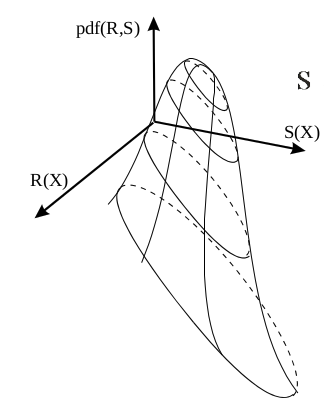
\includegraphics[scale=0.4]{./SurfWaves_figs/pdf_in_SR_plane.png}
\end{minipage}%
\begin{minipage}{.5\textwidth}
 \flushleft
  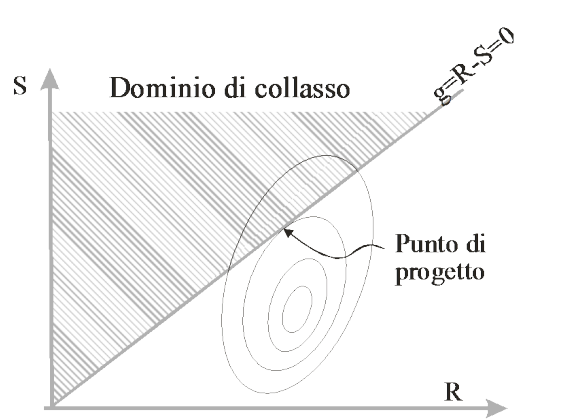
\includegraphics[scale=0.4]{./SurfWaves_figs/collapse_zone_in_SR_plane.png}
\end{minipage}
\caption{Probability density function in the $S-R$ plane, where $S$ is the Load and $R$ is the resistance. The grey zone is the failure zone}
  \label{fig:test3}
\end{figure}
The failure probability reads as the integral over the "grey" region (see Figure \ref{fig:test3}) of the pdf function. To compute this probability, it is required to know the cumulate probability density function in the region $g\rbkt{\mathbf{X}}=R\rbkt{\mathbf{X}}-L\rbkt{\mathbf{X}}< 0 $ until the design point, that stands on the surface $g\rbkt{\mathbf{X}}=R\rbkt{\mathbf{X}}-L\rbkt{\mathbf{X}}= 0$. Thus it is claimed to know:
\begin{itemize}
\item[-]the coordinates of the design point;
\item[-] the probability density function and the relative cumulate density function;
\item[-] the expression of the \textit{collapse function} $g\rbkt{\mathbf{X}}= R\rbkt{\mathbf{X}}-L\rbkt{\mathbf{X}}= 0 $, which in general is an hyper-surface of dimension $n-1$.
\end{itemize}
The above requirements holds for every domain in which we are representing the pdf, whatever it is the $\rbkt{L\rbkt{\mathbf{X}},R\rbkt{\mathbf{X}}}$ plane, or the $n$-dimensional space $\R^n$ containing the $\textbf{X} = \cbkt{x_{1}, x_{2},..., x_{n}}$ variables or any derived transformed variables $\textbf{Z} = \cbkt{z_{1}, z_{2},..., z_{n}}$. The approximation of the Level 2 methods are thus based on two fundamental points:
\begin{itemize}
\item the transformation of the base variables $\mathbf{X}$ into uncorrelated \textbf{normalized Gaussian} random variables $\mathbf{Z}$;
\item the approximation in a neighbourhood of the design point $\mathbf{X}^{*}$ (in the new uncorrelated Gaussian reference this point will be $\mathbf{Z}^{*}$) of the collapse functions with linear or quadratic functions, as
\begin{equation}\label{level2complete}
\mathbf{g}\rbkt{\mathbf{Z}}=\mathbf{g}\rbkt{\mathbf{Z}^{*}}+\mathbf{A}\rbkt{\mathbf{Z}-\mathbf{Z}^{*}}+\mathbf{B}\rbkt{\mathbf{Z}-\mathbf{Z}^{*}}^{2}.
\end{equation}
\end{itemize}
Various techniques have been proposed to transform the variables $\mathbf{X}$ into $\mathbf{Z}$. On one hand, this procedure strongly simplifies the definition of the probability density function, as it will indeed be a multivariate Gaussian random variable with diagonal variance (i.e. equal among all the dimension), that is a spherical symmetric function; on the other hand, the same transformation complicates the functional form of the Limit state surface $\mathbf{g}\rbkt{\mathbf{Z}}=0$. In order to minimize the error, this transformation must be applied in a neighbourhood of the design point, which is however not explicit, and hence an iterative procedure to determine it have to be applied. 
\subsection{First Order Reliability Method}
The most simple Level 2 analysis is the one performed with a first order approximation of equation $\eqref{level2complete}$, that is imposing $A$ equal to the gradient of $\mathbf{g}$ and $B\equiv0$, thus simplifying the equation as
\begin{equation}\label{FORM}
\mathbf{g}\rbkt{\mathbf{Z}}=\mathbf{g}\rbkt{\mathbf{Z}^{*}}+\left.\nabla\mathbf{g} \right|_{\mathbf{Z}^{*}}\rbkt{\mathbf{Z}-\mathbf{Z}^{*}}.
\end{equation}
\begin{figure}[t]
\centering
  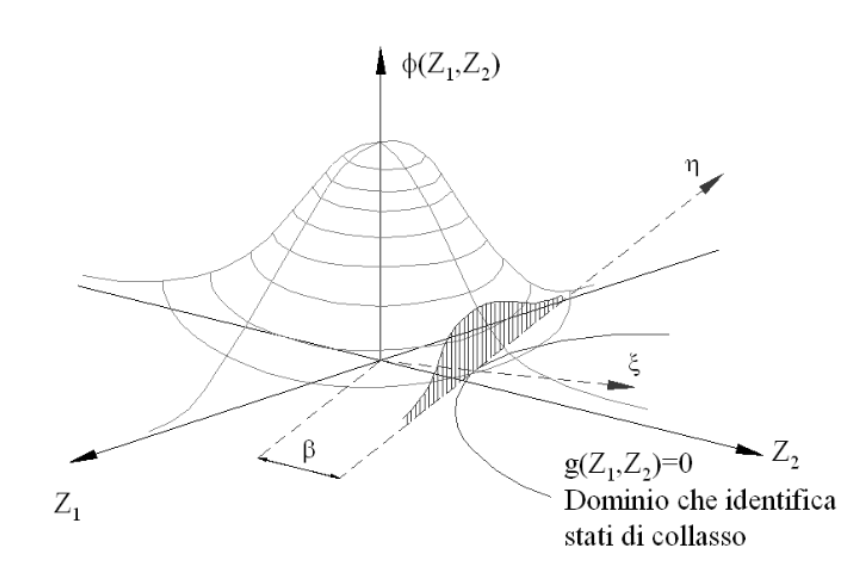
\includegraphics[scale=0.35]{./SurfWaves_figs/Hasofer_Lind_Method_approximations.png}
\caption{Graphical representation of the FORM method}
  \label{fig:test4}
\end{figure}
From Figure \ref{fig:test4} it can be seen that if the Limit State curve $\mathbf{g}\rbkt{\mathbf{Z}}=0$ is regular enough, thanks to the transformation of $\mathbf{X}$ in $\mathbf{Z}$ the design point $\mathbf{Z}^{*}$ is also the closest point on $\mathbf{g}\rbkt{\mathbf{Z}}=0$ to the origin. Furthermore, thanks to the radial symmetry of the multivariate Gaussian, the maximum slope of the pdf is over every radial line passing through the origin. This trivial thing has indeed a deep impact on the procedure: once the direction $\xi$ has been chosen as the direction of least distance from the curve to the origin, which will also be a direction of maximum growth of the probability density function, defining the \textbf{marginal probability} among $\xi$, this will also be a normalized Gaussian random variable. The collapse probability will be a function of the distance from the origin $\beta$ alone, and can be estimates, as easily can be seen from Figure \ref{fig:test5} as
\begin{equation}
\P_{f}=\int_{-\infty}^{-\beta}\varphi\rbkt{\xi}\,d\xi=\Phi\rbkt{-\beta},
\end{equation}
where $\Phi$ is the Cumulative Normal distribution. It is trivial now to understand that to evaluate $\P_{f}$ is necessary just the design point.
\begin{figure}[t]
\centering
  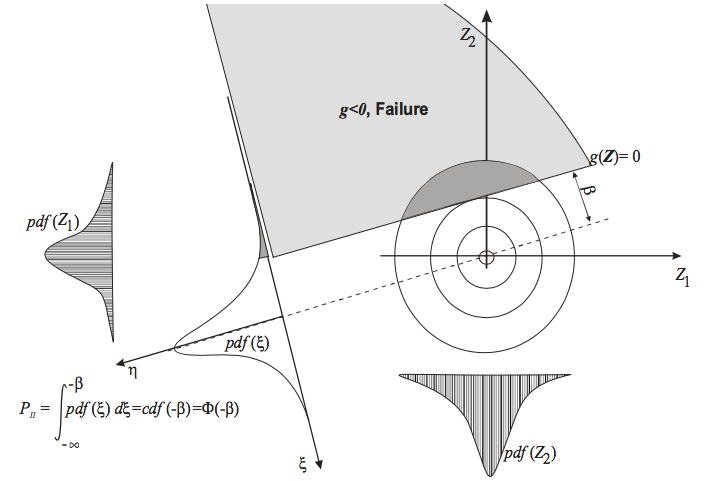
\includegraphics[scale=0.5]{./SurfWaves_figs/2_dimensional_case.png}
\caption{Bird-eye view of the Figure \ref{fig:test4}}
  \label{fig:test5}
\end{figure}
The steps to follow in order to evaluate the failure probability with the FORM scheme are thus the following
\begin{itemize}
\item[-]define the variables $X_{i}$: their distribution, mean and variance;
\item[-]transform the variables $X_{i}$ into uncorrelated normalized Gaussian $Z_{i}$;
\item[-]compute for each variable $Z_{i}$: $\frac{\partial \mathbf{g}}{\partial Z_{i}} ~ ~ ~  i = 1,...,n$;
\item[-]compute the cosine director 
 $
 \alpha_i = \frac 
	{- \frac {\partial g(Z_1,...,Z_n)} {\partial Z_i}}
	{
		\sqrt{
		\sum_{j=1}^n 
			(\frac {\partial g(Z_1,...,Z_n)} 
							{\partial Z_j})^2
		}
	} 
	~ ~ ~ i=1,...,n
 $
\item[-]compute $\beta$ by solving $g(\beta ~ (\alpha_1, ..., \alpha_n)) = 0;$
\item[-]compute the failure probability $P_f = \Phi (-\beta) $ 
\end{itemize}

\section{A case of study: The water level Load}
In the following study, it is investigated the probability of the sea water level to overcome a fixed height. The associated failure function $g$ has the form:
\begin{equation}
g=R-L
\end{equation}
where $R$ and $L$ represent the \textit{Resistance} and the \textit{Load} respectively. The Resistance is described by the \textit{coastal structure height} $d$ that is considered to be constant as a reasonable approximation for a coastal defence (not just a dune height). The Load reads as:
\begin{equation}
L = T + S + R
\end{equation}
where $T$, $S$ and $R$ represent the sea level contributes due to \textit{tide}, \textit{surge} and \textit{run-up} respectively. The Run-up is expressed by the formula:
\begin{equation*}
R=1.1~\cbkt{0.35b_{f}\sqrt{H_{o}L_{o}}+0.5\sqrt{H_{o}L_{o}\rbkt{0.004 + 0.563~b_{f}^{2}}}}
\end{equation*}
where $b_{f}$ is the slope assumed to be constant $b_{f} = 0.1$. In order to obtain uncorrelated variables, the following transformation operates on the wavelength:
\begin{equation*}
L_{o} = \frac {H_{o}} {S_{w}}
\end{equation*}
where $S_{w}$ represents the wave steepness.
After the transformation, the Run up writes as
\begin{equation*}
R=1.1~\cbkt{0.35b_{f}\sqrt{\frac {H_{o}^2} {S_{w}}}+0.5\sqrt{\frac {H_o^{2}} {S_{w}}\rbkt{0.004 + 0.563b_f^{2}}}}.
\end{equation*}
The failure event is represented by the condition
\begin{equation*}
g < 0.
\end{equation*}
or more extensively by
\begin{equation}
g=R-L=d - T - S - 1.1~\cbkt{0.35b_{f}\sqrt{\frac {H_{o}^2} {S_{w}}}+0.5\sqrt{\frac {H_o^{2}} {S_{w}}\rbkt{0.004 + 0.563b_f^{2}}}} < 0.
\end{equation}
\subsection{Mathematical expressions and parameters}
By following the lines of section $2$, the input variables are:
\begin{itemize}
\item[-] $X_1=T$ with normal probability density function (pdf)
\begin{equation*}
\Phi_{X_1}\rbkt{X_1} = \frac{1}{\sigma \sqrt{2 \pi}}\exp\cbkt{- \frac{\rbkt{X_{1} - \mu_{T}}^2} {2 \sigma_{T}^{2}}}
\end{equation*}
and cumulative density function (CDF)
\begin{equation*}
D\rbkt{X_{1}} = \frac{1}{\sigma_{X_{1}}\sqrt{2 \pi}}\int_{-\infty}^{X_{1}} \Phi_{X_{1}}\rbkt{X_{1}'}d X_{2}' = \rbkt{1+\erf\rbkt{X_1}}
\end{equation*}
\item[-] $X_2=S$ with log-normal pdf 
\begin{equation*}
\Phi_{X_{2}}\rbkt{X_{2}} =\frac{1}{\sigma_{S} \sqrt{2 \pi} X_{2}}\exp\rbkt{ \frac{\rbkt{\ln X_{2} - \mu_{S}}^2}{2 \sigma_{S}^{2}}}
\end{equation*}
and CDF
\begin{equation*}
D\rbkt{X_{2}}= \frac{1}{2}\sbkt{1 + \erf \rbkt{\frac {\ln \rbkt{X_{2}} - \mu_{X_{2}}}{\sigma_{X_{2}} \sqrt{2}}}}
\end{equation*}
\item[-] $X_3=H_o$ with Gumbel pdf 
\begin{equation*}
\Phi_{X_{2}} =\frac{1}{\beta}\exp\sbkt{\frac { x - \alpha}{\beta} -  \exp \rbkt{\frac {x - \alpha} {\beta}}}
\end{equation*}
where 
\begin{equation*}
\mu_{H_{o}} = \alpha - \gamma \beta 
			 , \quad \sigma_{H_{o}}^2  = \frac{1}{6}\pi^{2} \beta^{2} ,\quad 
			 \gamma = ~ \text{Euler-Mascheroni costant}
\end{equation*}
and CDF
\begin{equation*}
D\rbkt{X_{3}} = 1 - \exp\rbkt{-\exp\rbkt{\frac {X_{3} - \alpha}{\beta}}}
\end{equation*}
\item[-]$X_{4}=S_{w}$ with lognormal distribution
\begin{equation*}
\Phi_{X_{4}}\rbkt{X_{4}} = \frac{1}{\sigma_{S_{w}} \sqrt{2 \pi} X_{4}}\exp\sbkt{- \frac{(\ln X_{4} - \mu_{S_{w}})^2}{2 \sigma_{S_{w}}^2}}
\end{equation*}
and CDF
\begin{equation*}
D\rbkt{X_{4}} = \frac{1}{2}\sbkt{ 1 + \erf \rbkt{\frac {\ln \rbkt{X_{4}} - \mu_{X_{4}}}{\sigma_{X_{4}} \sqrt{2}}}}
\end{equation*}
			.
\end{itemize}
$ $
The gradients of the failure function $g(Z_1,..,Z_4)$ at the design point are calculated by:
\begin{itemize}
\item[]$\frac{\partial g}{\partial Z_1} = - \sigma_T$
\item[]$ \frac{\partial g}{\partial Z_2} = - \sigma_S$
\item[]$ \frac{\partial g}{\partial Z_3} = 
	-(37\sigma_{H_o}(1/(\mu_{S_{w}} + Z_4 \sigma_{S_{w}}))^{1/2})/400 $;
	\item[]$ \frac{\partial g}{\partial Z_4} = (37 \sigma_{S_{w}} (1/(m(4) + Z_4 \sigma_{S_{w}}))^{3/2} 
		(\mu_{H_o} + Z_3\sigma_{H_o}))/800;$.
\end{itemize}
so the director cosines are immediate to compute (see section 2). 
\\\\
By following the steps described in paragraph $1.3.2$, in the next section, it is shown the code to:
\begin{itemize}
\item[-]obtain iteratively the approximate design point;
\item[-]compute the probability of failure at the design point.
\end{itemize}


